\documentclass[12pt,longbibliography]{article}
\usepackage[utf8]{inputenc}
\usepackage[T1]{fontenc}
\usepackage[catalan]{babel}
\usepackage[a4paper, margin=2.7cm]{geometry}

\usepackage{amsmath, amsthm, amsfonts, amssymb}
\newtheorem{thm}{Theorem}[section]
\newtheorem{cor}[thm]{Corollary}
\newtheorem{lem}[thm]{Lemma}
\newtheorem{prop}[thm]{Proposition}
\theoremstyle{definition}
\newtheorem{defn}[thm]{Definition}
\theoremstyle{remark}
\newtheorem{rem}[thm]{Remark}

\usepackage{mathrsfs} 
\usepackage[colorlinks=true,linkcolor=blue,citecolor=blue,urlcolor=blue,breaklinks]{hyperref}

\usepackage{bbm} 

\usepackage{hyperref}
\usepackage{graphicx}
\graphicspath{ {Imatges portada/} }

\title{Big Query}
\author{Anna Salazar}

\renewcommand{\contentsname}{Índex}
\renewcommand{\figurename}{Figura}
\renewcommand{\tablename}{Taula}

\begin{document}
\begin{titlepage}
\maketitle

\vspace{140mm}

\par
\raisebox{-.5\height}{
\includegraphics[width=6cm]{fme}}%
\hfill
\raisebox{-.5\height}{
\includegraphics[width=6cm]{UB}}%
\par

\end{titlepage}

\tableofcontents

\pagebreak

\pagenumbering{arabic}

\section{Què és BigQuery?}

BigQuery és un motor d’anàlisi de macrodades (Big Data) que permet executar consultes SQL al núvol sobre les dades emmagatzemades en aquest, sense importar el volum de les dades ni el tipus de consultes que es volen fer. El motor de consulta és capaç de treballar sobre terabytes de dades en qüestió de segons, i sobre petabytes en pocs minuts. Avui en dia, les empreses estan adoptant cada cop més la presa de decisions basades en dades i fomentant una cultura oberta en la qual les dades no estan aïllades dins dels departaments. BigQuery, en proporcionar els mitjans tecnològics per a promoure un canvi cultural cap a l’agilitat i l’obertura, realitza un paper molt important en l’augment del ritme de la innovació.

\vspace{2mm}

Treballar amb dades a BigQuery implica 3 aspectes principals: l’emmagatzemament, la incorporació de les dades i la consulta d’aquestes, Google s’encarrega de tota la resta. Com BigQuery és un servei totalment gestionat, no és necessari configurar ni instal·lar res en el nostre ordinador i, pel mateix motiu, no necessitem un administrador de la base de dades. Simplement, podem entrar en el nostre projecte de Google Cloud des del nostre navegador i començar a analitzar.

\vspace{2mm}

Pel que fa a l’emmagatzemament, les dades es guarden en una taula estructurada, la qual cosa significa que es pot utilitzar l’SQL estàndard per a facilitar la consulta i l’anàlisi de dades. BigQuery és perfecta pel Big Data perquè gestiona tot aquest emmagatzemament i està proveïda d’operacions d’escalabilitat que funcionen de forma automàtica sense que l’usuari s’hagi d’involucrar,  per la qual cosa mai haurem de preocupar-nos per la grandària de les dades amb els quals treballem. Part de la consideració de disseny darrere de BigQuery és animar als usuaris a centrar-se en els coneixements en lloc de la infraestructura. Quan s’introdueixen les dades a BigQuery no és necessari pensar en els diferents tipus d’emmagatzemament, ni en els seus avantatges pel que fa a velocitat i cost; l’emmagatzemament està totalment gestionat.

\vspace{2mm}
\noindent
Per a més informació sobre BigQuery, es pot consultar la pàgina de \href{https://cloud.google.com/bigquery/docs/introduction}{Google Cloud}.

\subsection{Per què hauríem d'utilitzar BigQuery en lloc d'altres eines?}

Una de les característiques més rellevants que presenta BigQuery és que es tracta d'una plataforma sense servidor, és a dir, que els servidors s'executen en segon pla, sense l'intervenció de l'usuari. A més, presenta una alta disponibilitat, la qual cosa es tradueix en que no cal preocupar-se per la caiguda dels servidors, ja que la plataforma s'encarrega d'això. Per últim, BigQuery també té propietats d'escalabilitat automàtica que fan possible gestionar fins a petabytes de dades. Aquestes característiques no estan disponibles a la majoria de plataformes d'emmagatzament de dades tradicionals, cosa que fa destacar BigQuery entre moltes.

\vspace{2mm}

Com en molts altres magatzems de dades, BigQuery és capaç de treballar amb moltes fonts de dades diferents. Podem pujar les dades des del nostre propi sistema d'arxius, de Google Cloud Storage, de Google Drive i de moltes fonts més. Després de fer-ho, es poden consultar aquestes dades utilitzant SQL estàndard o SQL heretat, el rendiment en qualsevol cas és excel·lent. Els resultats de les consultes solen emmagatzemar-se en la memòria cau durant 24 hores, de manera que les següents execucions d'aquesta consulta només hauran d'obtenir les dades de la memòria cau en lloc de fer-ho del disc. 


\pagebreak

\section{Creació i treball amb conjunts de dades i taules}

\subsection{Configuració de la Plataforma de Google Cloud (GCP)}

\graphicspath{ {BigQuery/Imatges tutorial/} }

Per utilitzar aquesta eina d’anàlisi només ens caldrà crear un compte a Google Cloud i treballar a la zona de proves que ofereix Google per treballar de forma gratuïta.
Per fer servir la zona de proves (\textit{Sandbox}) seguirem els passos següents: 

1. En primer lloc, ens dirigim a la interfície d’usuari de \href{https://console.cloud.google.com}{BigQuery}. Des d'aquesta interfície es poden realitzar la majoria de les operacions.

\vspace{2mm}

2. Accedim al nostre compte de Google o creem un nou compte si encara no en tenim cap. Si és el primer cop que iniciem sessió a Google Cloud, haurem de marcar el país on som i acceptar les condicions de servei.

\vspace{2mm}

3. Un cop dins, podem veure com és l'espai de treball SQL. Hi ha una secció de l'Explorador a l'esquerra que ens permet navegar en projectes, conjunts de dades i taules.Per tal de fer servir la zona de proves, haurem de crear un projecte.

Introdueix un nom al teu projecte i fes clic a Create. En el nostre cas, hem anomenat el projecte \verb|el_meu_projecte|, i treballarem sobre aquest per il·lustrar el funcionament de la plataforma.

\vspace{2mm}
\begin{figure}[h!]
\par
\raisebox{-.5\height}{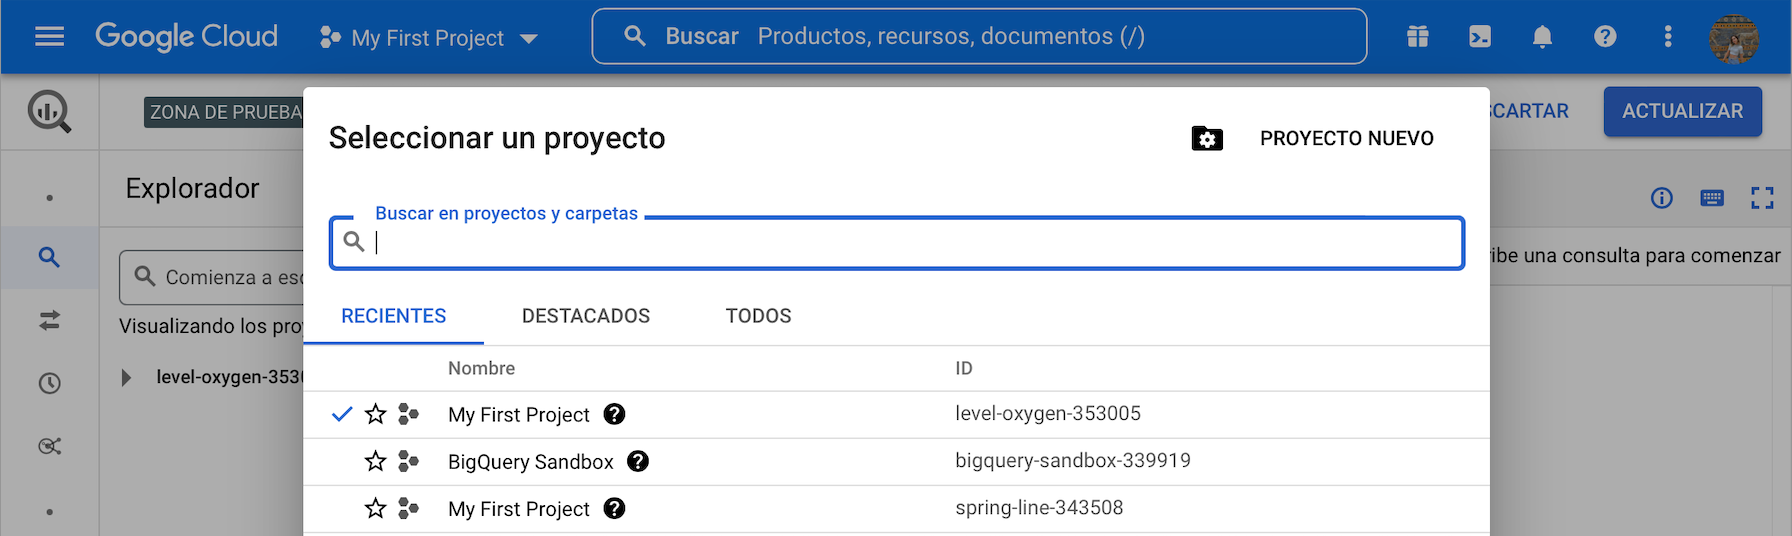
\includegraphics[width=7.25cm]{bq1}}%
\hfill
\raisebox{-.5\height}{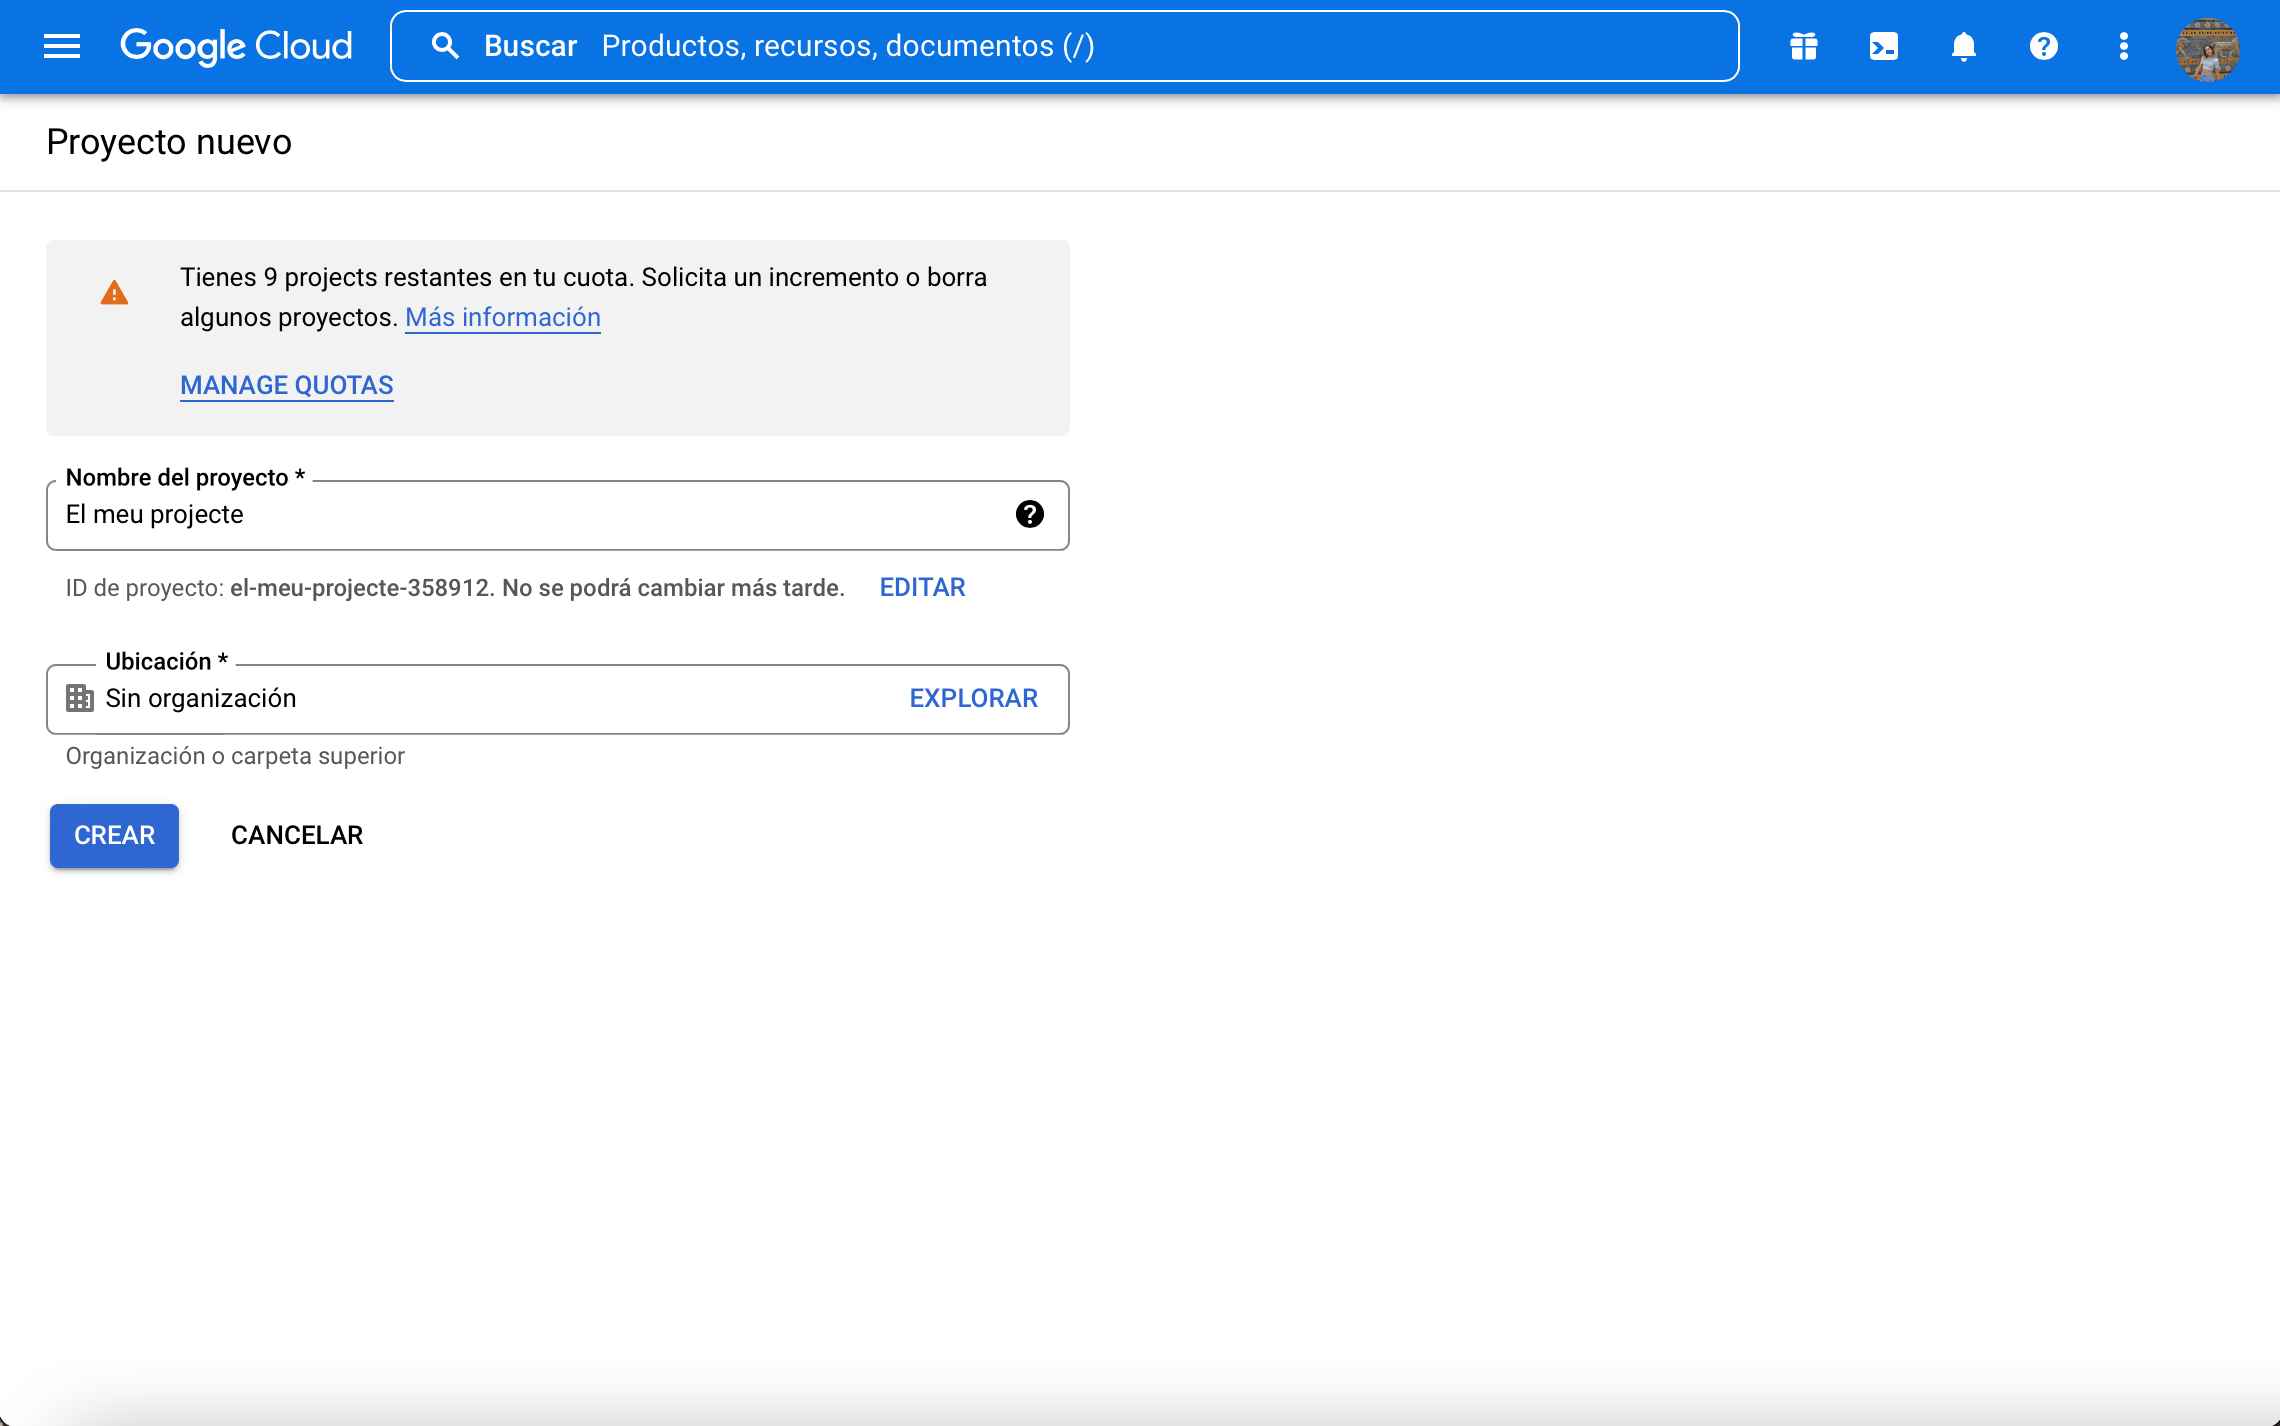
\includegraphics[width=7.25cm]{bq2}}%
\par
\caption{Creació d'un projecte}
\label{fig:bq1}
\end{figure}
\vspace{2mm}

4. Un cop creat el projecte, el navegador ens redirigigeix a la interfície web de BigQuery.

\vspace{2mm}

5. Ara ja podrem carregar o consultar dades en el nostre projecte sense cap compte de facturació adjunta.

\subsubsection{Limitacions}

Per a l’ús de la zona de proves gratuïta que ofereix Google, haurem de tenir en compte un seguit de limitacions.

\vspace{2mm}

En primer lloc, ens trobem amb un màxim de 10 Gb d’emmagatzemament i 10 Tb de consulta al mes. Al llarg d’aquest projecte no utilitzarem un volum de dades més gran ni sobrepassarem el límit d’espai de consulta, però s’han de tenir en compte aquestes limitacions si l’objectiu és treballar amb el format gratuït.

\vspace{2mm}

A més, ens trobem que tots els conjunts de dades tenen el temps de caducitat de la taula per defecte establerta en 60 dies. Per tant, totes les taules, vistes o particions de les taules caducaran automàticament passats els 60 dies.

\vspace{2mm}

Una altra característica destacable és que els projectes de la zona de proves no són compatibles amb:

- La transmissió de dades

- Sentència de llenguatge de manipulació de dades (DML)

- Servei de transferència de dades de BigQuery

\subsection{Creació d'un conjunt de dades}

Ara que ja coneixem les limitacions de la plataforma i disposem d'un projecte en el que crear un conjunt de dades, ha arribat el moment de crear un nou conjunt de dades dins d'un projecte. Es pot pensar en un conjunt de dades a \textit{BigQuery} com una agrupació lògica de taules. Alhora, diferents cojunts de dades s'integren en un mateix projecte. 

\vspace{2mm}

Per a crear-ne un, només s'ha de desplegar el menú i triar l'opció de crear un nou conjunt de dades. Tot seguit hi ha diversos detalls per al conjunt de dades que es poden establir. En primer lloc, hi ha l'opció de canviar el projecte que l'encabirà. Això farà que aparegui un navegador on es pot especificar el projecte. Una altra possibilitat serà escollir la ubicació de les dades. Això determina on s'aprovisionaran els recursos subjacents, com la computació i l'emmagatzematge, per al servei \textit{BigQuery}. Les consideracions a l'hora de triar una ubicació inclouran el rendiment per als usuaris finals, l'alta disponibilitat i també qualsevol restricció d'auditoria o compliment. I, per últim, es pot establir un temps d'expiració per defecte per a les taules dins d'un conjunt de dades.

\vspace{2mm}
\begin{figure}[h!]
\par
\raisebox{-.5\height}{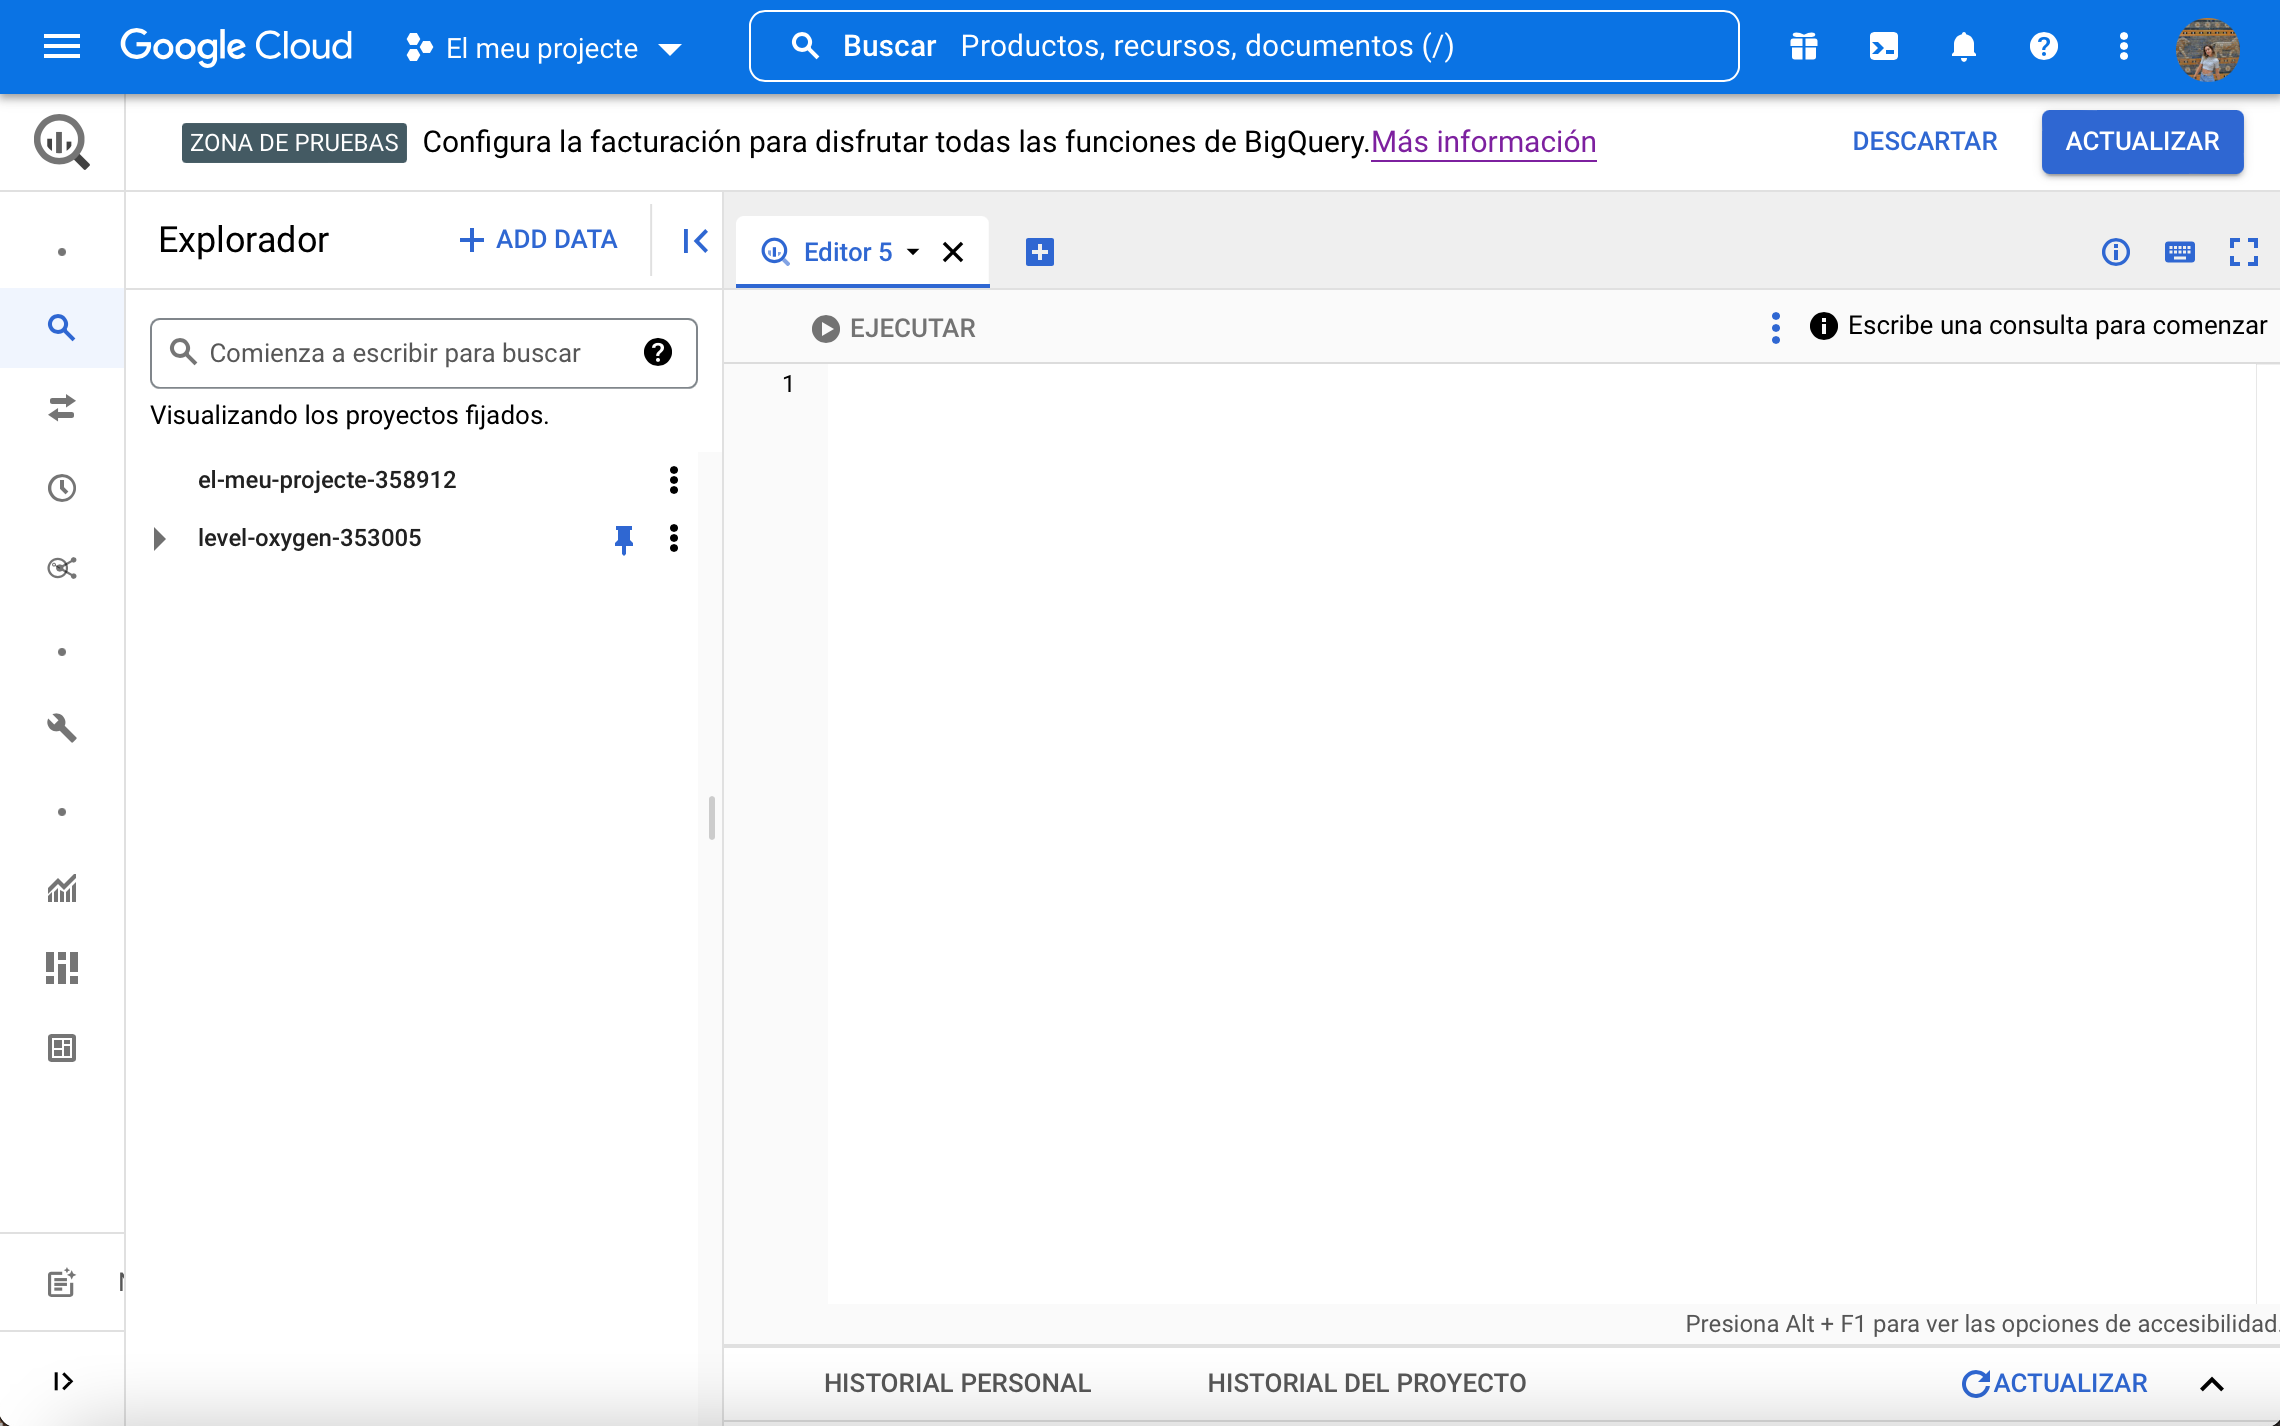
\includegraphics[width=7.25cm]{bq3}}%
\hfill
\raisebox{-.5\height}{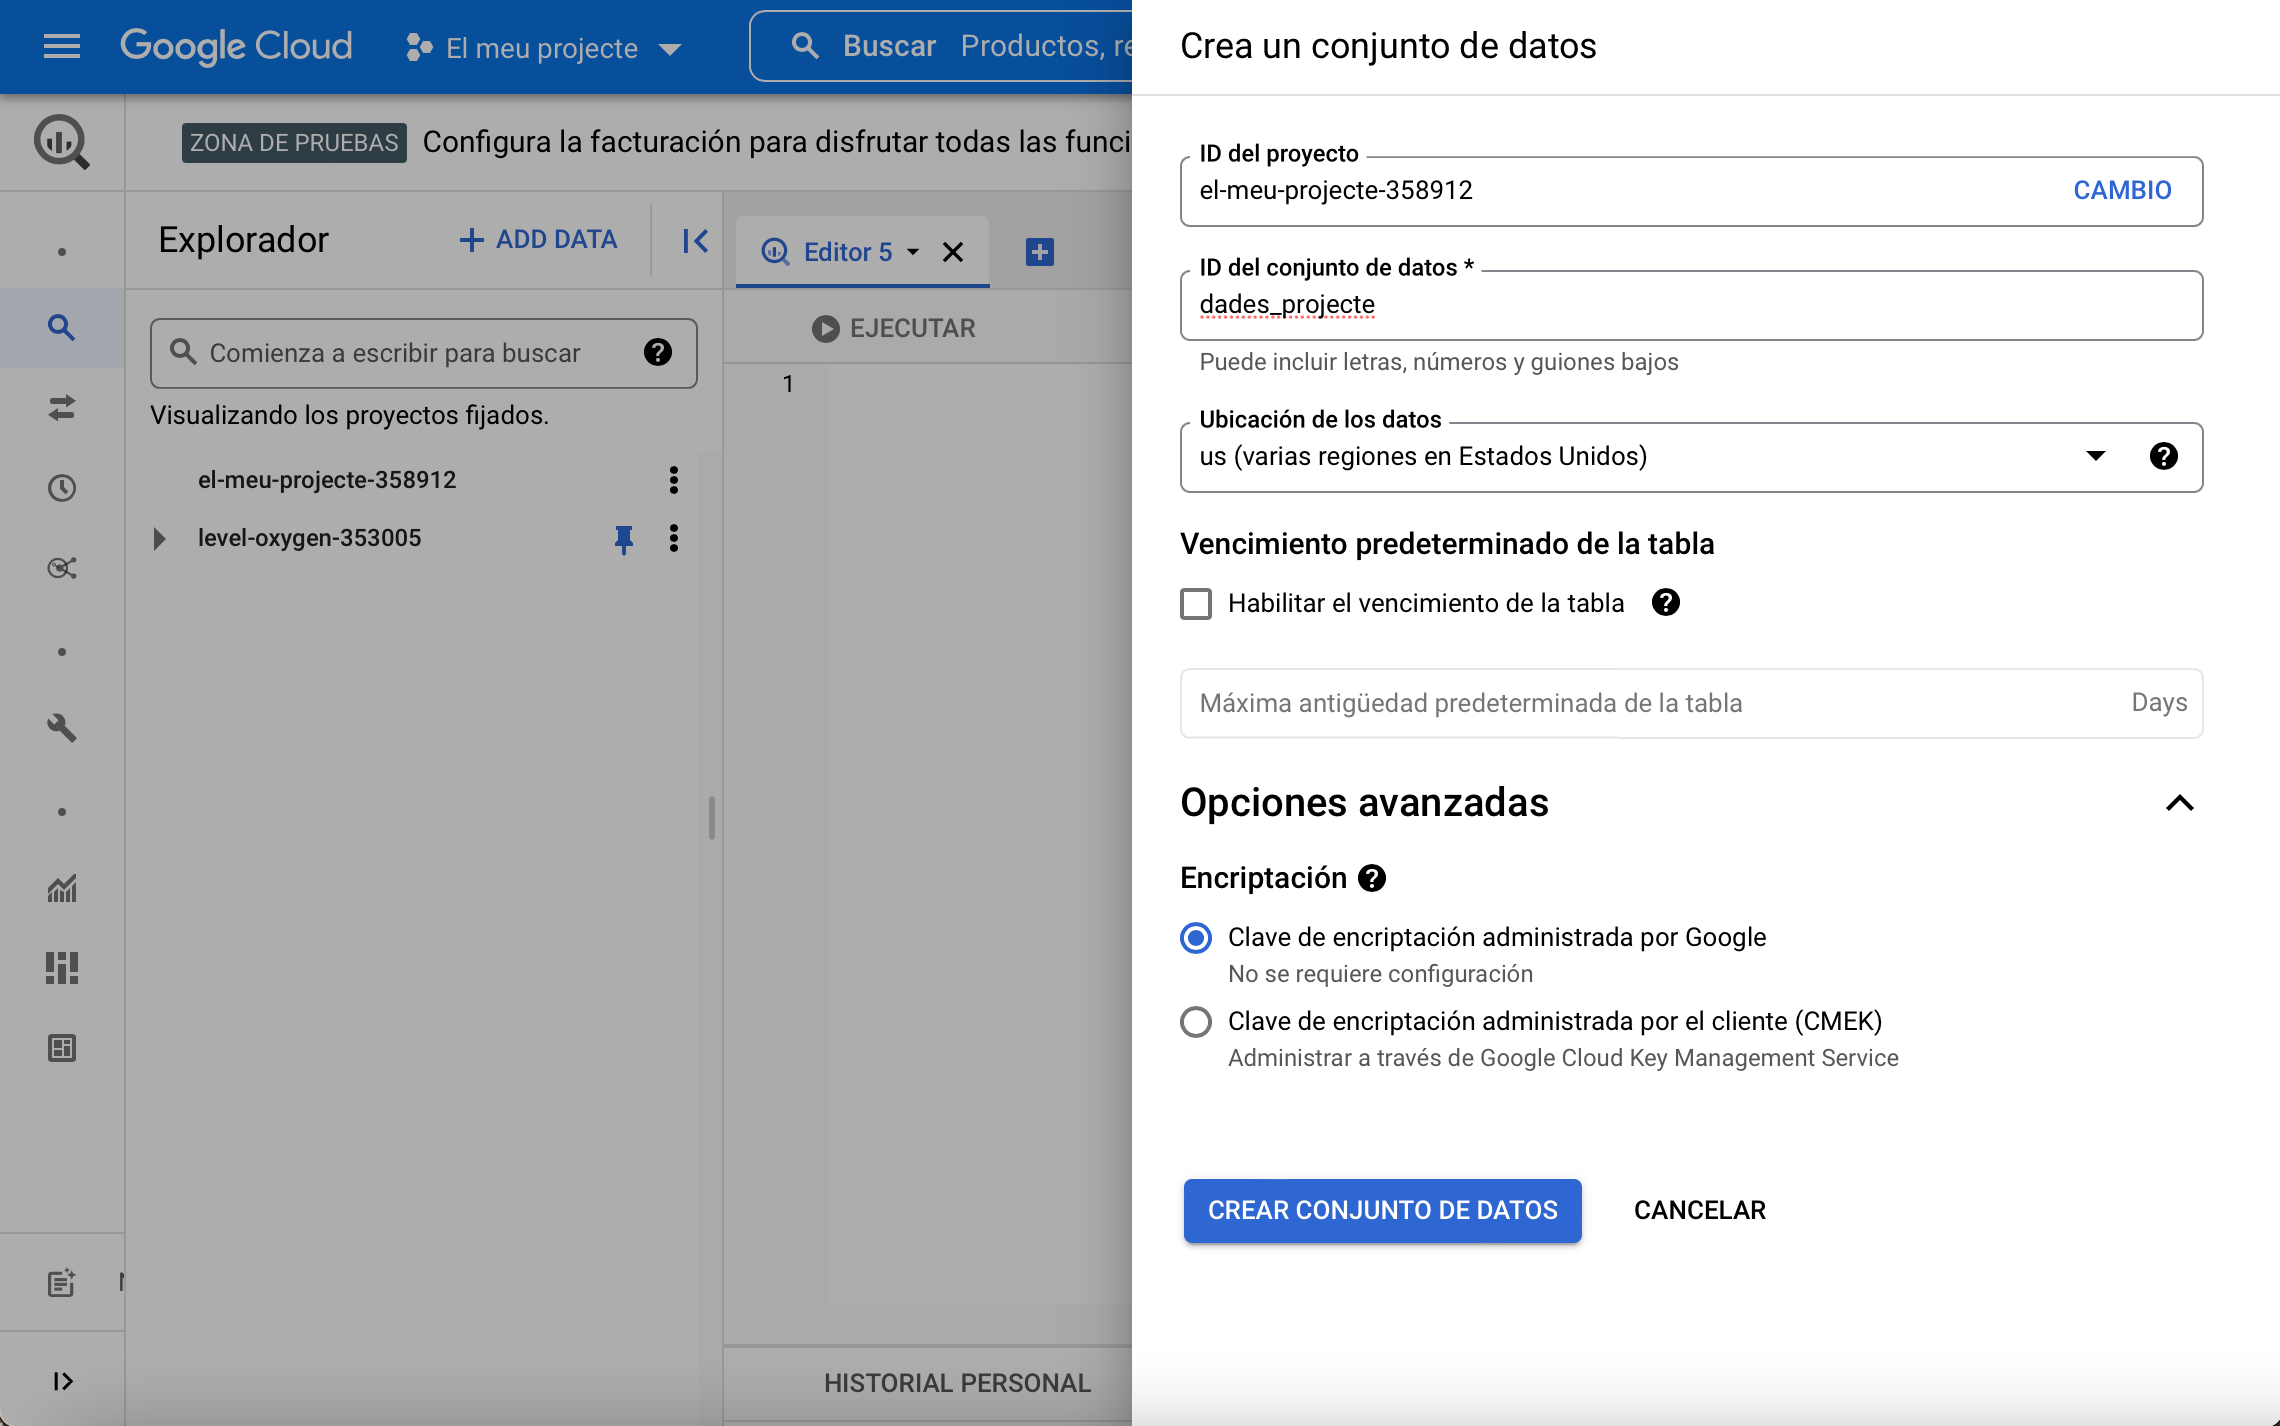
\includegraphics[width=7.25cm]{bq4}}%
\par
\caption{Creació d'un conjunt de dades}
\label{fig:bq3}
\end{figure}
\vspace{2mm}

Tal com es pot veure a la figura anterior, hem creat un nou conjunt de dades anomenat \verb|dades_projecte| que estarà ubicat en el projecte \verb|el_meu_projecte|, la ubicació de les dades la hem posat a diverses regions dels Estats Units i, per últim, no hem habilitat un temps de venciment de la taula, sinó que per defecte \textit{BigQuery} l'emmagatzemarà per 60 dies.

\vspace{2mm}
\begin{figure}[h!]
\begin{center}
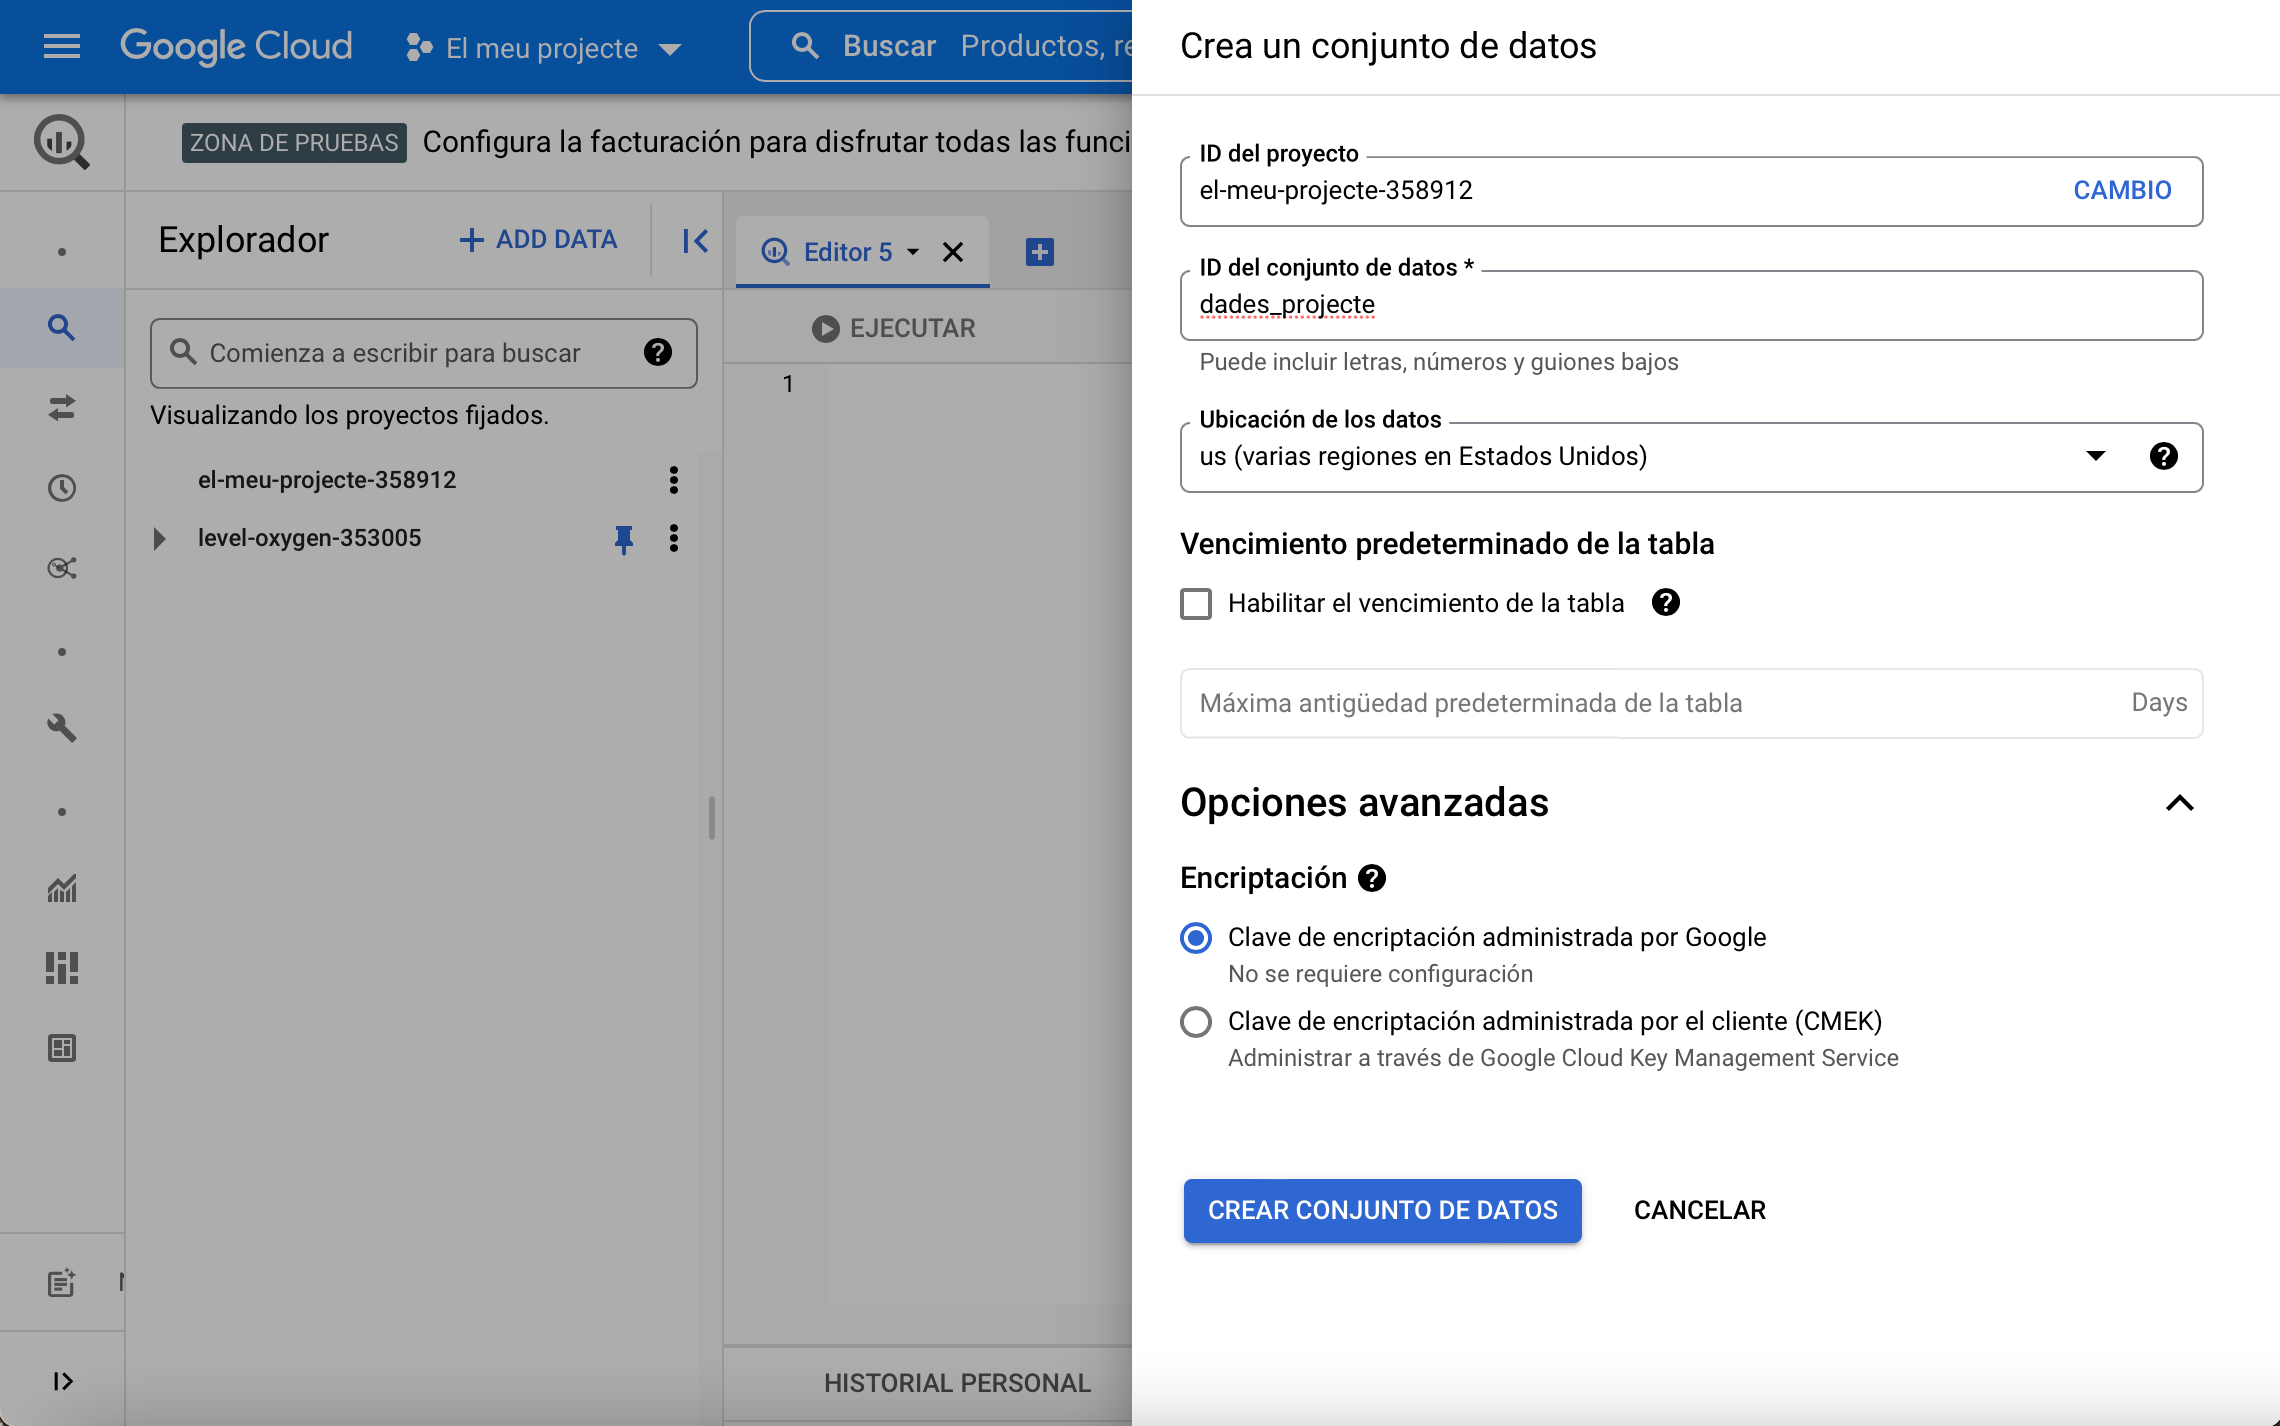
\includegraphics[width=10cm]{bq5}
\end{center}
\caption{Informació del conjunt de dades}
\label{fig:bq5}
\end{figure}
\vspace{2mm}

Un cop creat, el conjunt de dades \verb|dades_projecte| ara apareix dins de \verb|el_meu_projecte|, I ampliant això s'observa que no hi ha taules dins d'aquest. Ara, es pot donar un cop d'ull als detalls associats a aquest conjunt de dades. Des d'aquest menú, podem triar obrir-lo, moment en el qual la informació del conjunt de dades apareix a la dreta. Aquí podem confirmar l'identificador del conjunt de dades, que també assenyala el projecte en el qual s'ha creat el conjunt de dades, i després altres detalls que inclouen les hores de creació i modificació. 

\vspace{2mm}

A més, des d'aquesta finestra podrem compartir el conjunt de dades amb altres usuaris. Hi ha opcions per a copiar i eliminar aquest conjunt de dades. I després, a \textit{editar detalls}, podem reconfigurar el temps de caducitat de les taules, establir una descripció o afegir etiquetes. Per exemple, si volem marcar aquest conjunt de dades com a pertanyent a un equip, podem establir una etiqueta amb la clau d'equip i el valor corresponent. Després, quan guardem aquest conjunt de dades, les etiquetes apareixen a l'apartat de informació.

\subsection{Definició d'una taula de BigQuery des de la interfície d'usuari}

Després d'haver creat un conjunt de dades en un projecte, ja es pot crear una taula dins d'aquest conjunt de dades. Si tenim la informació del conjunt de dades, hauríem de veure aquesta opció per a crear una nova taula des d'aquí. Alternativament, podem dirigir-nos al projecte, després al conjunt de dades i triar l'opció de crear una taula. Apareixerà un formulari i tindrem l'opció d'especificar una font per a la nostra taula. Això ens permetrà extreure dades de fonts ja existents, com l'emmagatzematge en el núvol de Google o bé un arxiu dels nostres propis sistemes. La primera taula que crearem serà bastant simple. De fet, serà una taula buida, i es pot observar la seva creació a la figura ~\ref{fig:bq6}. 

\vspace{2mm}
\begin{figure}[h!]
\par
\raisebox{-.5\height}{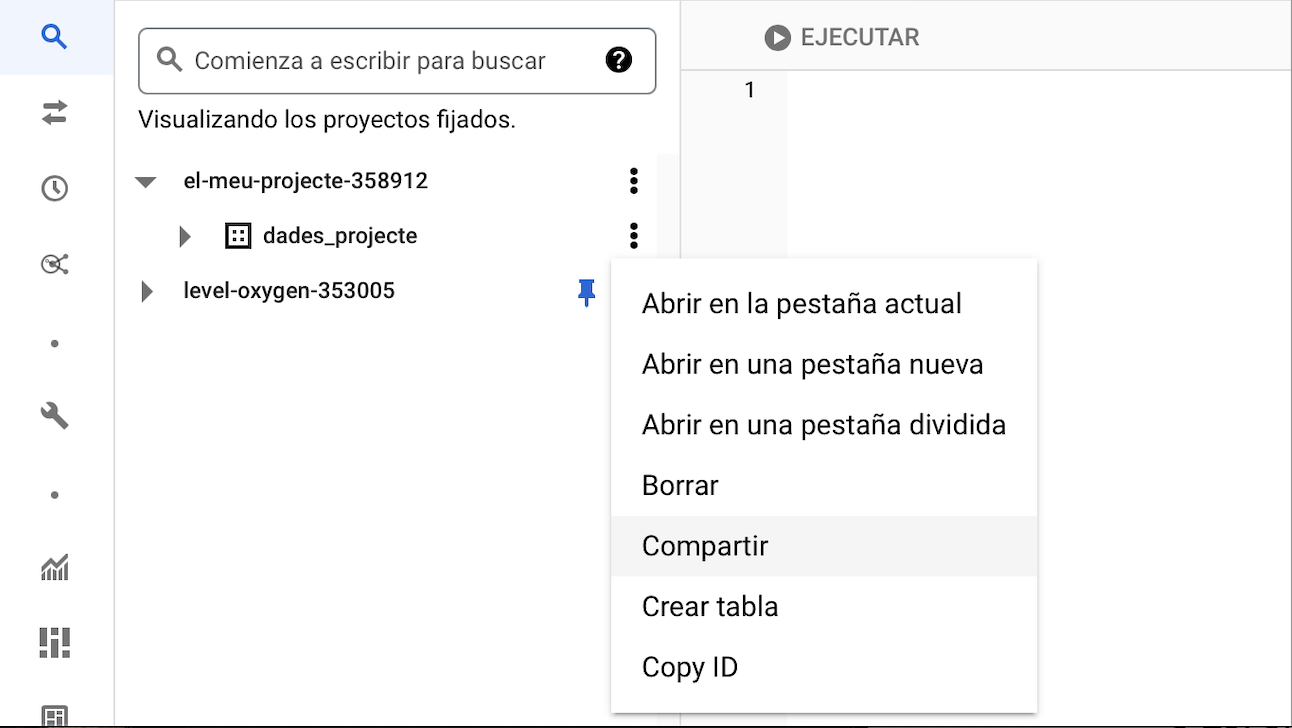
\includegraphics[width=7.25cm]{bq6}}%
\hfill
\raisebox{-.5\height}{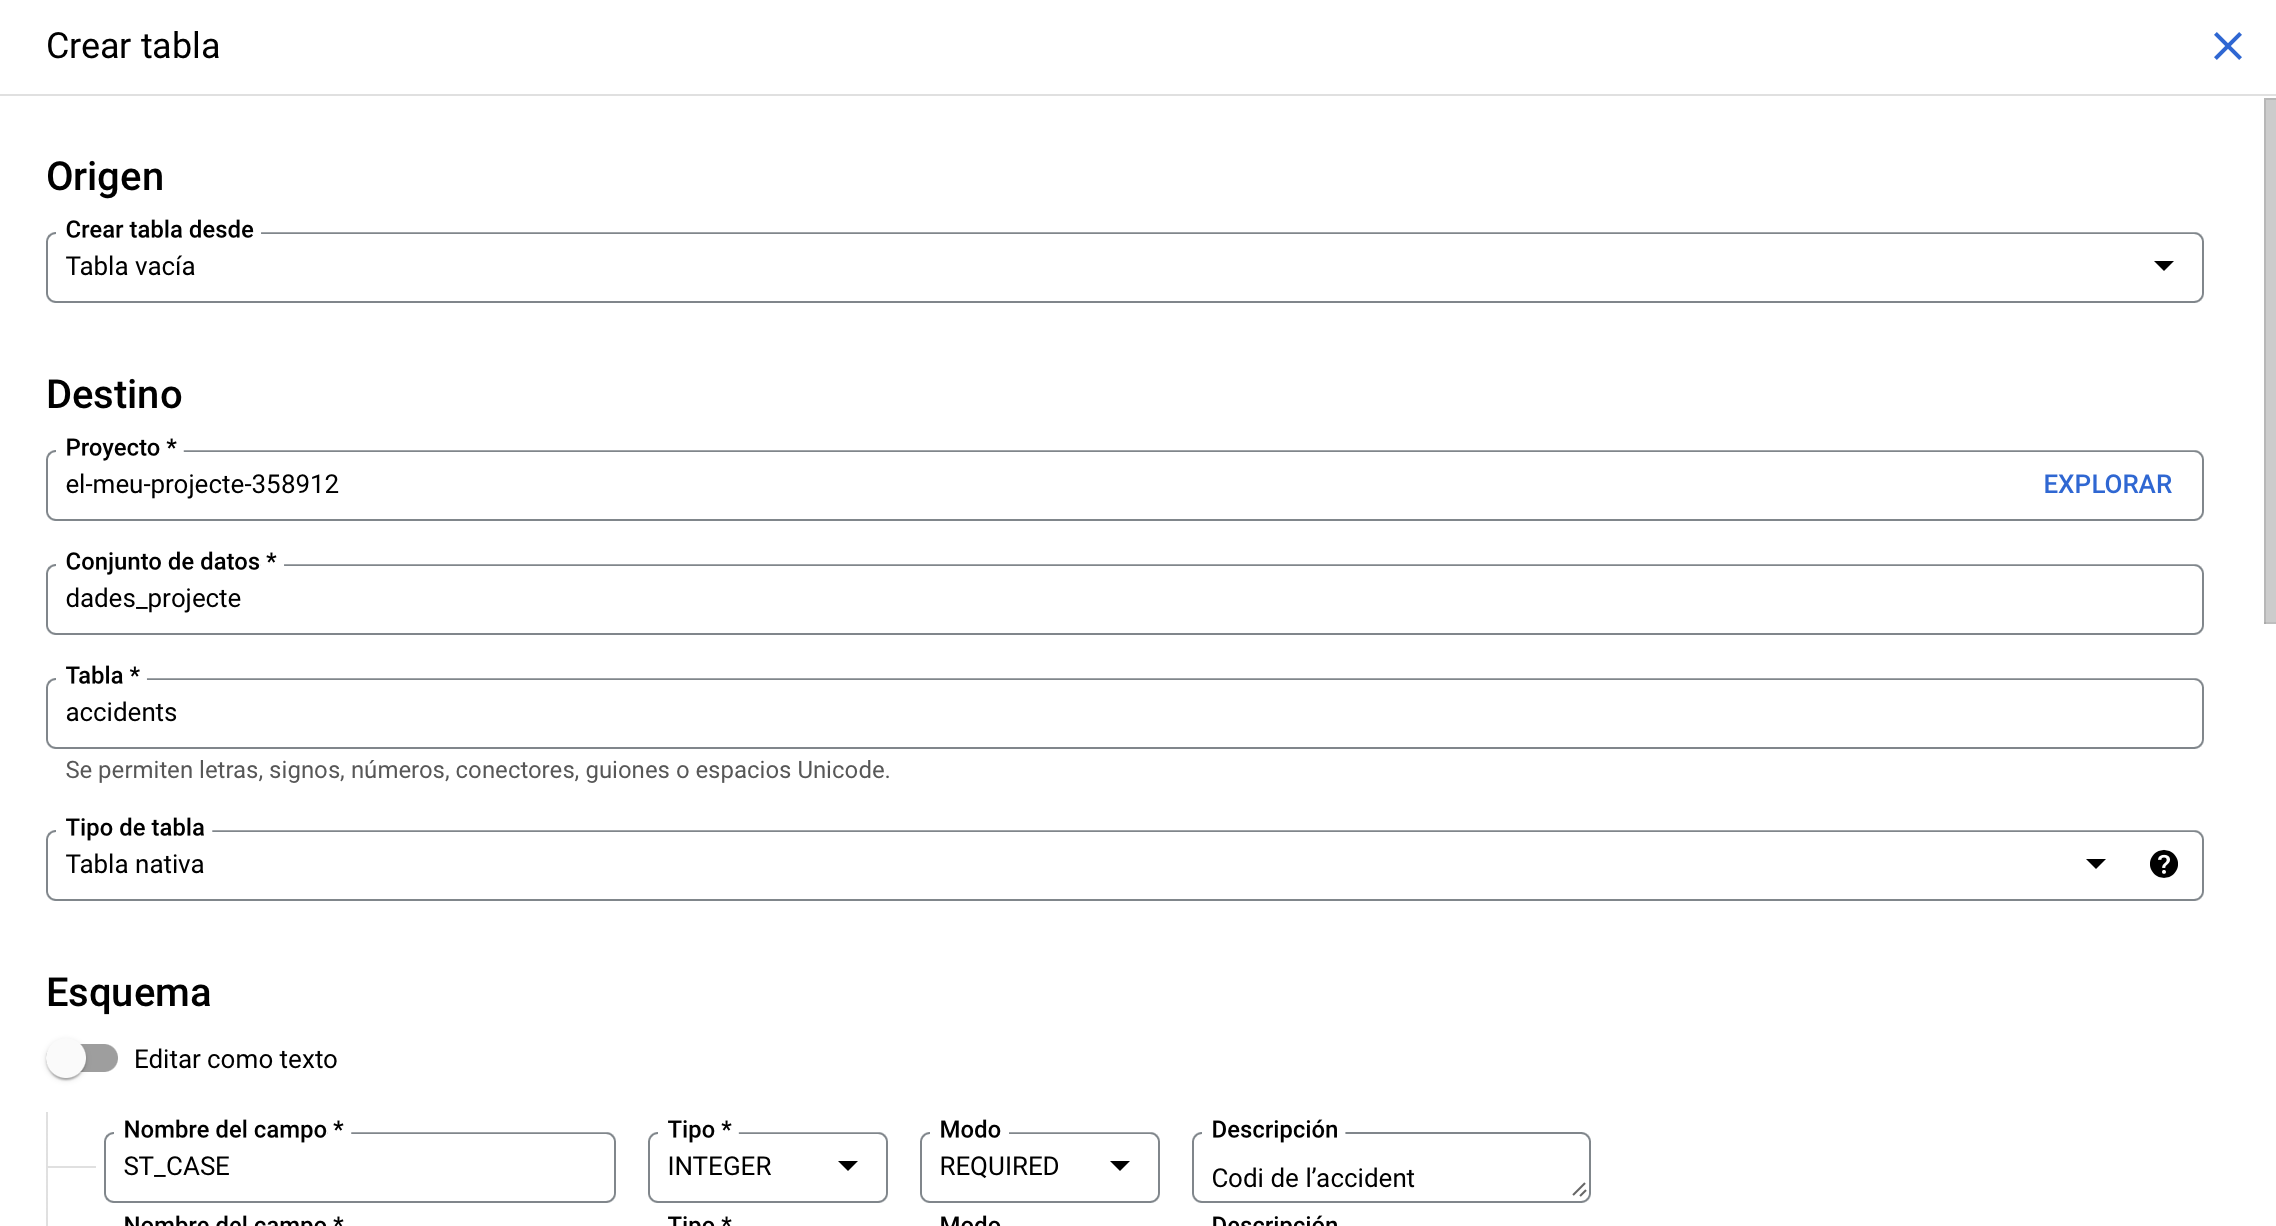
\includegraphics[width=7.25cm]{bq7 copia}}%
\par
\caption{Creació d'una taula}
\label{fig:bq6}
\end{figure}
\vspace{2mm}

A continuació, passem a la secció d'Esquema. Podem fer ús d'aquesta interfície per a establir les columnes de la nostra taula, incloent-hi els tipus i altres configuracions. La primera columna que definiré és l'identificador de l'accident, que s'anomenarà \verb|ST_CASE|. Per al tipus de variable, podem triar d'un menú, que inclou tots els tipus amb els quals ja estem familiaritzats. Quant a la manera (columna \textit{modo} a la figura ~\ref{fig:bq8}), aquesta determinarà si els valors d'aquesta columna poden ser nuls o si es requereix un valor, així com també podem establir que els valors siguin d'un tipus repetit com \textit{indistint}. Finalment, es pot escriure una descripció, que és opcional. 

\vspace{2mm}
\begin{figure}[h!]
\begin{center}
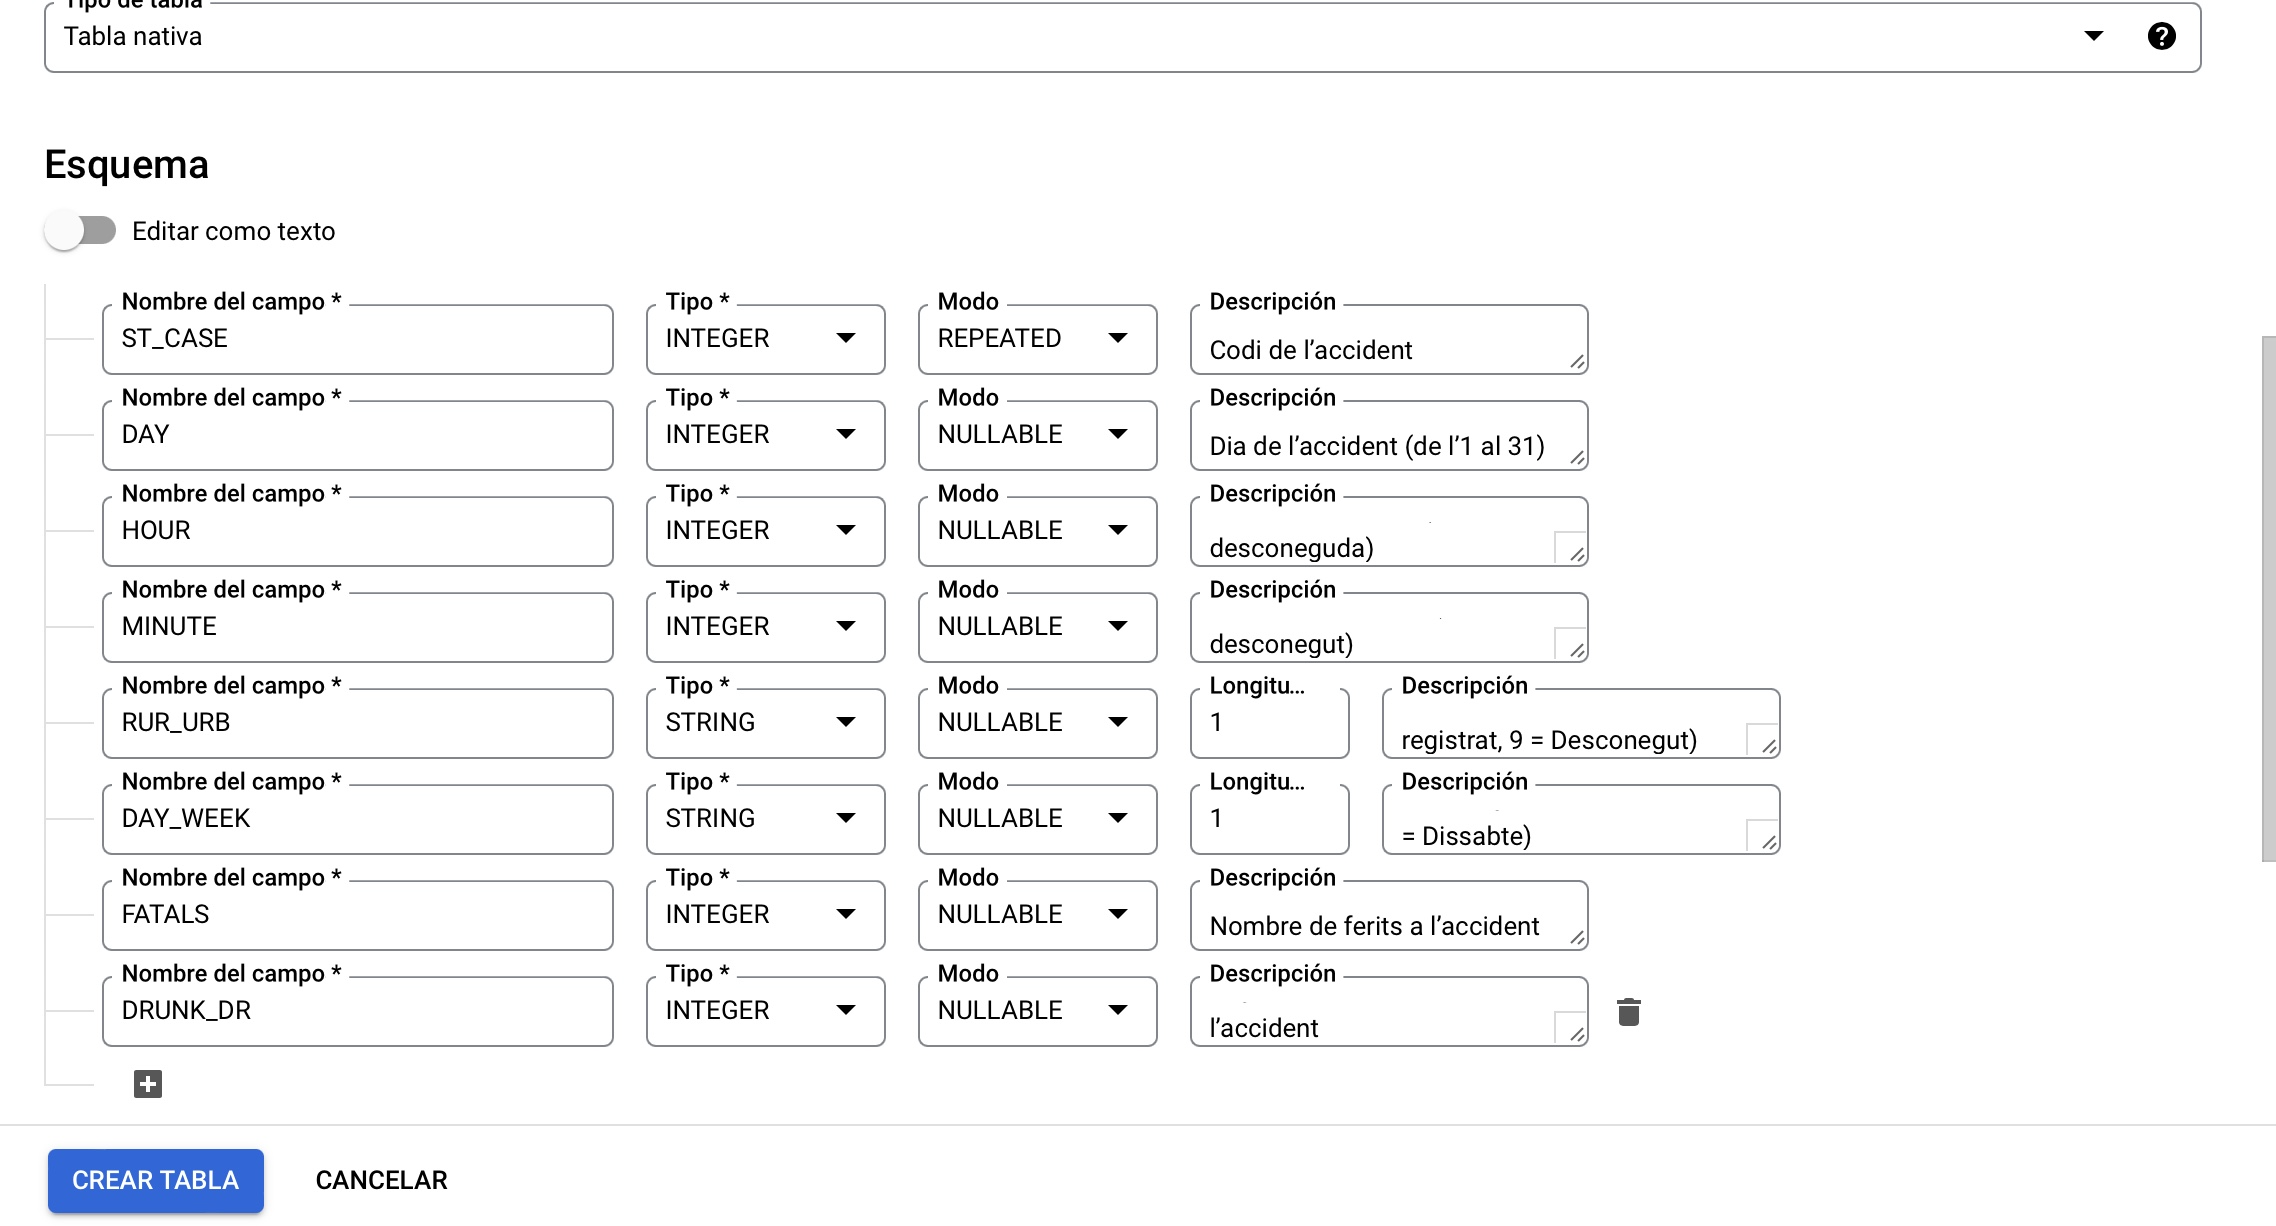
\includegraphics[width=10cm]{bq8}
\end{center}
\caption{Esquema de la nostra taula}
\label{fig:bq8}
\end{figure}
\vspace{2mm}

La taula ~\ref{tab:taula1} que acabem de crear està formada per 8 variables, 6 de les quals són numèriques i 2 categòriques, i es descriuen tal i com es pot veure a la taula següent:

\begin{table}[h]
\resizebox{\textwidth}{!}{%
\begin{tabular}{|l|l|l|}
\hline
Variable  & Tipus      & Descripció                                                                                                        \\ \hline
ST\_CASE       & Numèrica & Codi de l'accident                                                                                   \\ \hline
DAY       & Numèrica & Dia de l’accident (de l’1 al 31)                                                                                    \\ \hline
HOUR      & Numèrica   & Hora de l’accident (99 = desconeguda)                                                                               \\ \hline
MINUTE    & Numèrica   & Minut de l’accident (99 = desconegut)                                                                               \\ \hline
RUR\_URB  & Categòrica & Informació sobre la localització (1 = Rural, 2 = Urbà, 6 = Via no classificada, 8 = No registrat, 9 = Desconegut)   \\ \hline
DAY\_WEEK & Categòrica & Dia de la setmana (1 = Diumenge, 2 = Dilluns, ..., 7 = Dissabte)                                                    \\ \hline
FATALS    & Numèrica   & Nombre de ferits a l’accident                                                                                       \\ \hline
DRUNK\_DR & Numèrica   & Nombre de conductors beguts involucrats a l’accident                                                                \\ \hline
\end{tabular}%
}
\caption{Especificacions de la taula Accidents}
\label{tab:taula1}
\end{table}

\subsubsection{Afegir dades a una taula de BigQuery senzilla}

Ara que hem creat una taula de consulta, podem centrar-nos en treballar amb ella. Per a això, ens desplaçarem cap avall i donarem un cop d'ull al primer esquema de la taula (a la figura ~\ref{fig:bq9}). I aquí és on podem donar un cop d'ull a alguna informació interessant. Més enllà de la identificació de la taula, que es troba a l'esquerra de la figura, també podem comprovar la grandària de la taula a la dreta, que ens donarà una indicació de la quantitat de dades que es processaran, si anéssim a executar consultes contra ella. La grandària d'emmagatzematge a llarg termini assenyala les dades a les quals no s'ha accedit en els últims 90 dies, i després, per descomptat, tenim les hores de creació i modificació juntament amb la ubicació de les dades de la taula, que correspon a la ubicació de l'alimentador de dades que va ser reemplaçat. Des d'aquesta interfície, també podem editar els detalls existents d'aquesta taula. Aquí podem establir un temps de caducitat en cas que vulguem anul·lar el que s'ha establert en el nivell del conjunt de dades. També tenim l'opció d'establir una descripció o afegir etiquetes.

\vspace{2mm}
\begin{figure}[h!]
\par
\raisebox{-.5\height}{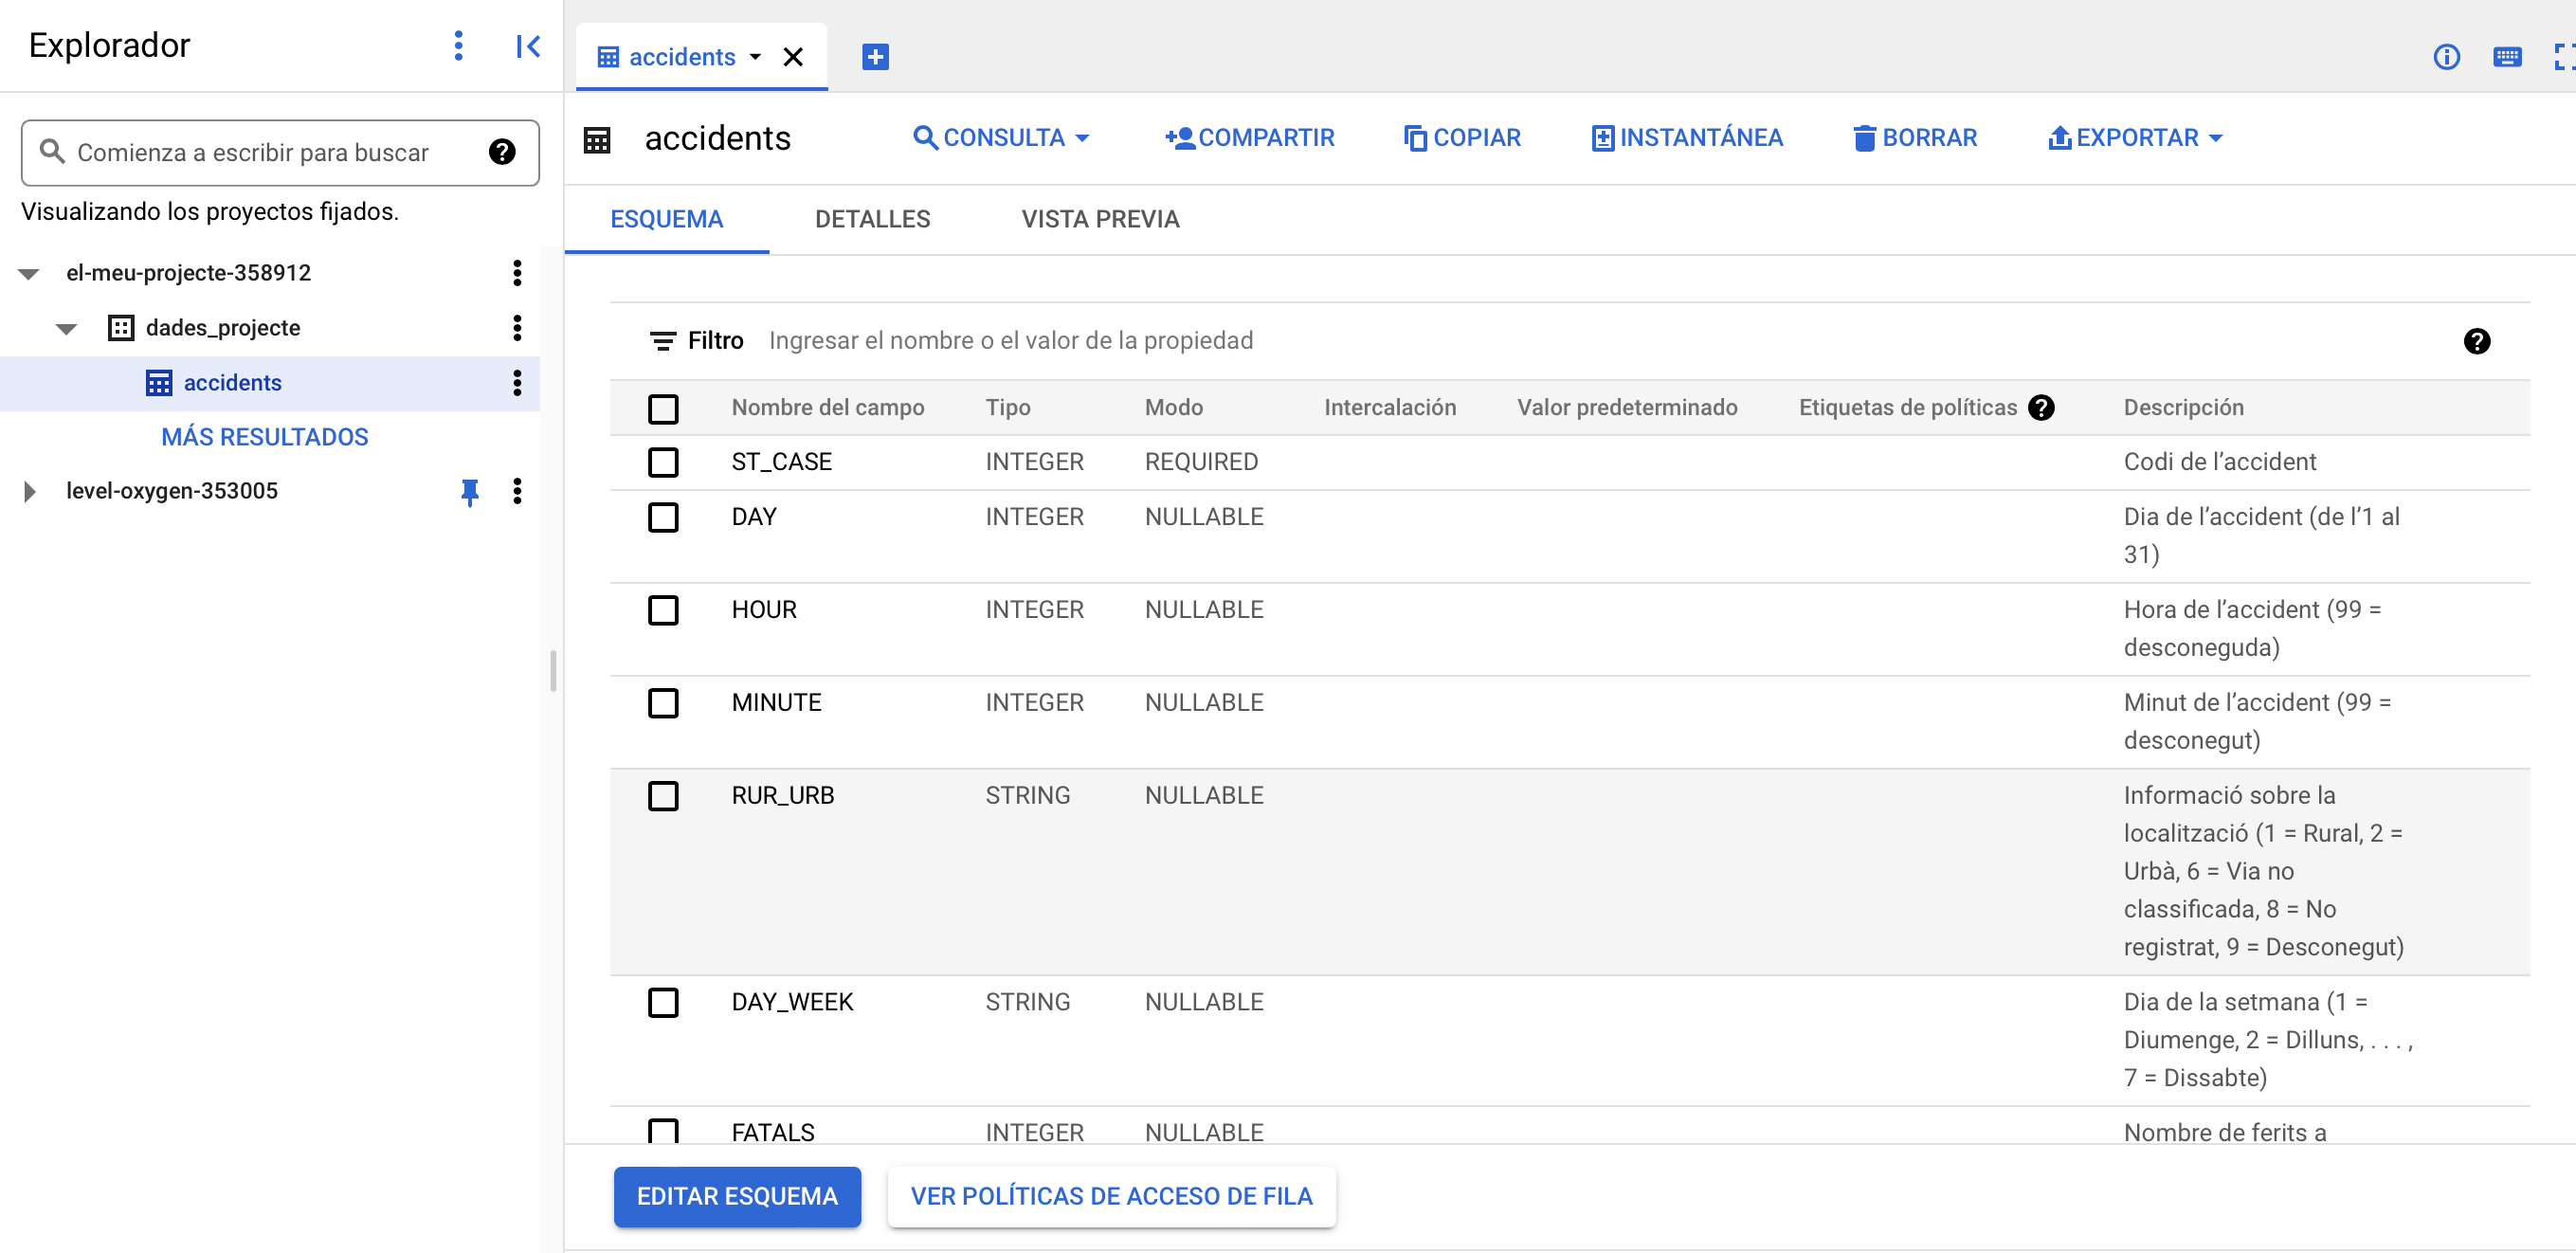
\includegraphics[width=7.25cm]{bq9}}%
\hfill
\raisebox{-.5\height}{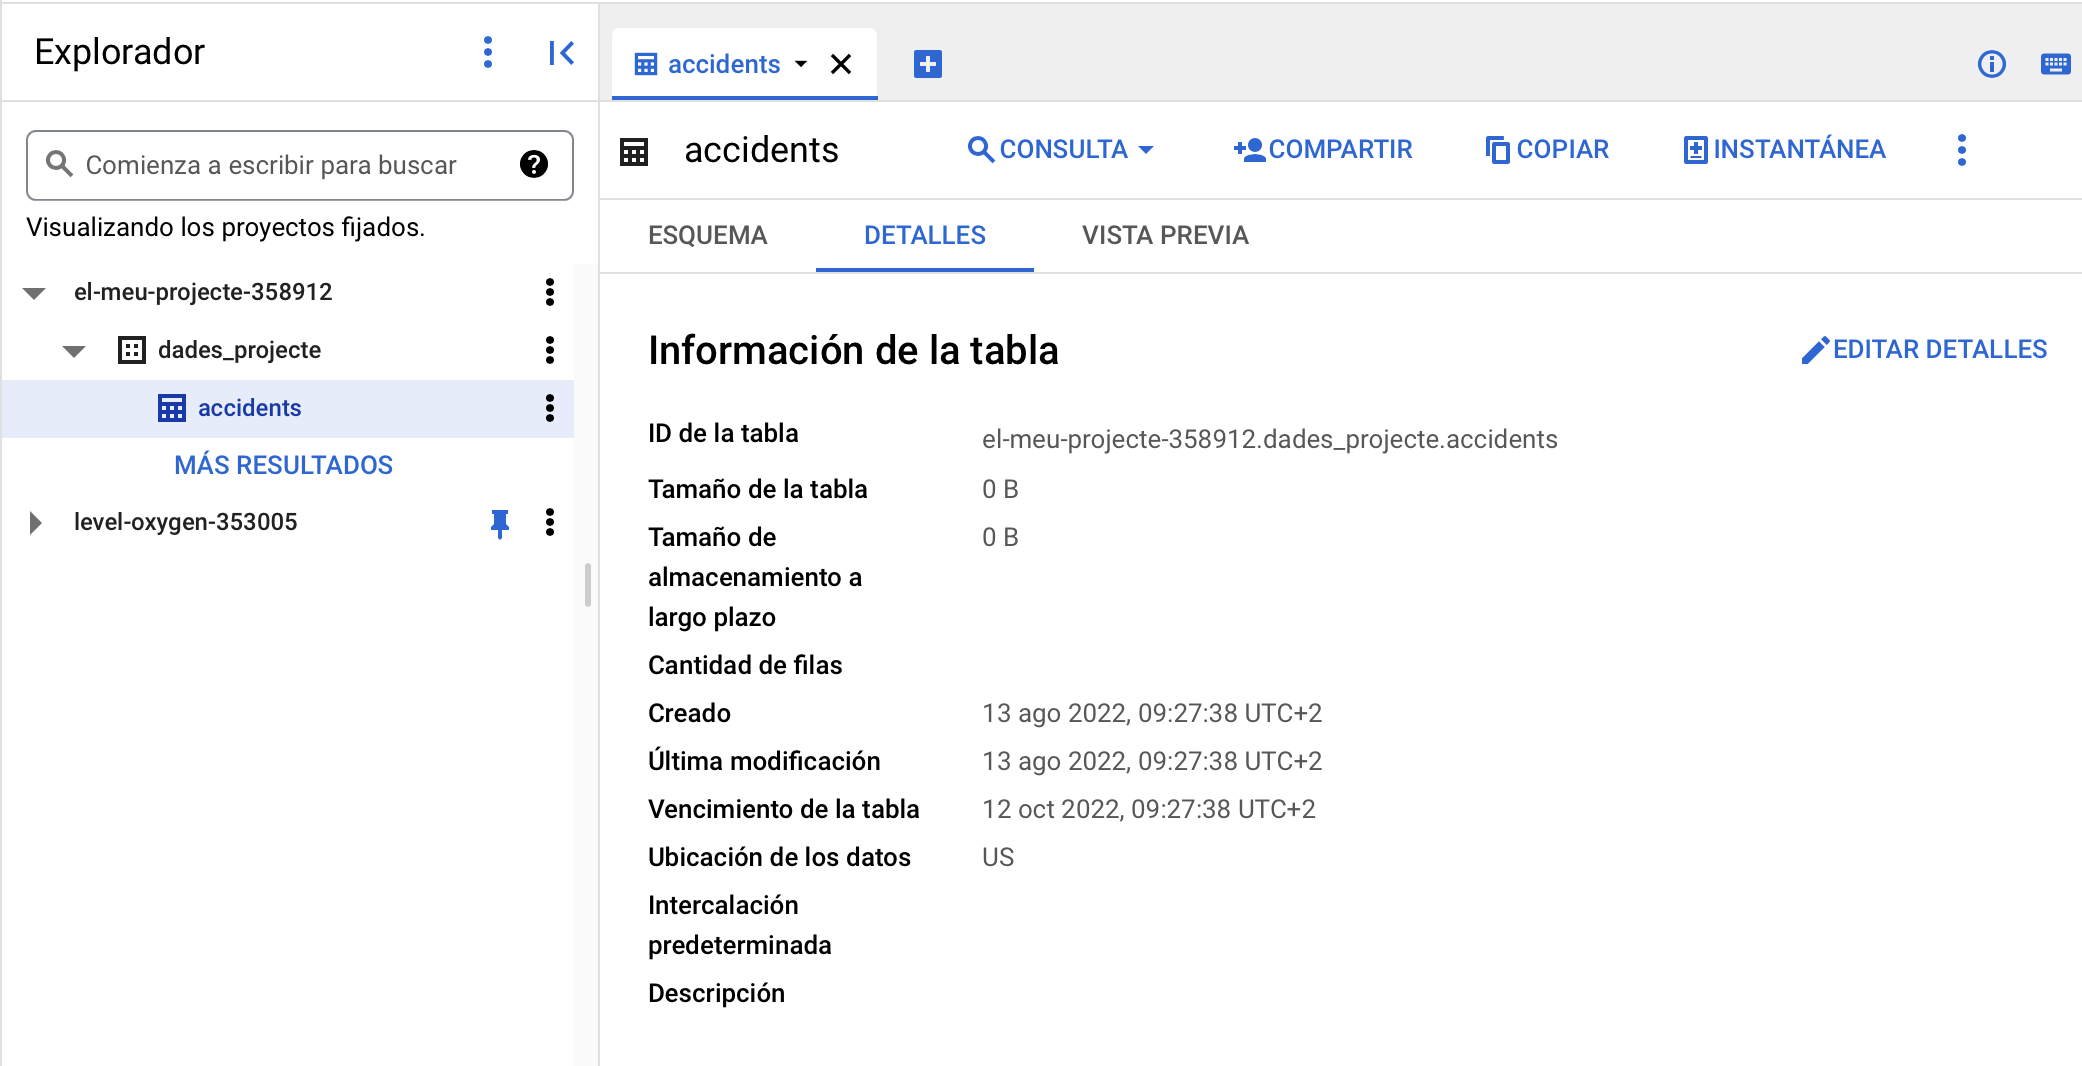
\includegraphics[width=7.25cm]{bq10}}%
\par

\caption{Detalls de la taula}
\label{fig:bq9}
\end{figure}
\vspace{2mm}

Una altra característica que podem consultar és la vista prèvia de la taula, i com és lògic, veurem que aquesta encara no conté dades, ja que simplement hem creat l'esquema de la taula, sense inserir cap dada en aquesta. Podrem afegir dades a partir d'una simple consulta a la taula.

\begin{verbatim}
INSERT INTO `el-meu-projecte-358912.dades_projecte.accidents` 
(ST_CASE, DAY, HOUR, MINUTE, RUR_URB, DAY_WEEK, FATALS, DRUNK_DR)
VALUES (20055, 1, 20, 55, "1", "3", 3, 0);
\end{verbatim}

Comencem amb "insert into", seguit de la taula en la qual s'ha de realitzar la inserció. Per a això, utilitzem parèntesi, i dins dels parèntesis, utilitzem la sintaxi, data set *name *dot *able *name, que en el meu cas és, *loony* underscore university.students. A continuació, en la línia número dos, podem especificar els noms de les columnes per a les quals s'afegiran valors, així que, com s'ha especificat, cadascuna de les cinc columnes presents en la taula, i després, seguit de la paraula clau values, especifiquem entre parèntesi, els propis valors. Observi's que en les consultes grans, podem utilitzar cometes dobles en especificar cadenes. També hi ha una altra informació interessant aquí per a la que minimitzaré el panell de l'explorador. Notaràs que hi ha un missatge que assenyala que es processaran zero bytes, quan executem aquesta consulta. Ara, seguirem endavant i executar aquesta consulta, i sembla que la inserció va ser un èxit, atès que una fila s'ha afegit a la taula dels estudiants. Per a confirmar-ho, executem una consulta més, concretament, un select from loony university.students. Significativament, obtenim un missatge que diu que, en executar aquesta consulta, es processaran 60 bytes de dades, assenyalant el cost que es produirà. Efectivament, l'única fila ha estat retornada, i fins i tot en els resultats de la consulta, obtenim la confirmació que s'han processat 60 bytes. El temps d'execució de la consulta també apareix aquí.

\subsection{Càrrega de dades per crear una taula de BigQuery}

Hem vist que és possible crear una taula buida i després emplenar-la amb dades amb sentències INSERT, ara explorarem un cas d'ús més comú per als usuaris de BigQuery en el qual es crea una taula a partir de dades existents. Per a això, ens dirigirem al conjunt de dades \verb|dades_projecte| i triarem crear una nova taula. I aquesta vegada, la font no serà una taula buida, sinó que carregarem un arxiu CSV del nostre propi sistema d'arxius per al qual es pot seleccionar l'opció de càrrega. Això no obstant, els tipus d’arxiu que podem importar han de ser del tipus CSV, JSON, Avro o Parquet, principalment. Hi ha algunes restriccions quant a la grandària de l'arxiu que podem pujar. Per tant, aquest ha de romandre dins dels 100 MB.  Procedim llavors a navegar pels nostres sistemes d'arxius per a l'arxiu a pujar. I després navegar fins a \verb|accidents.csv|. Una vegada que l'arxiu ha estat seleccionat, el format de l'arxiu s'ha establert automàticament en CSV. 

\vspace{2mm}
\begin{figure}[h!]
\par
\raisebox{-.5\height}{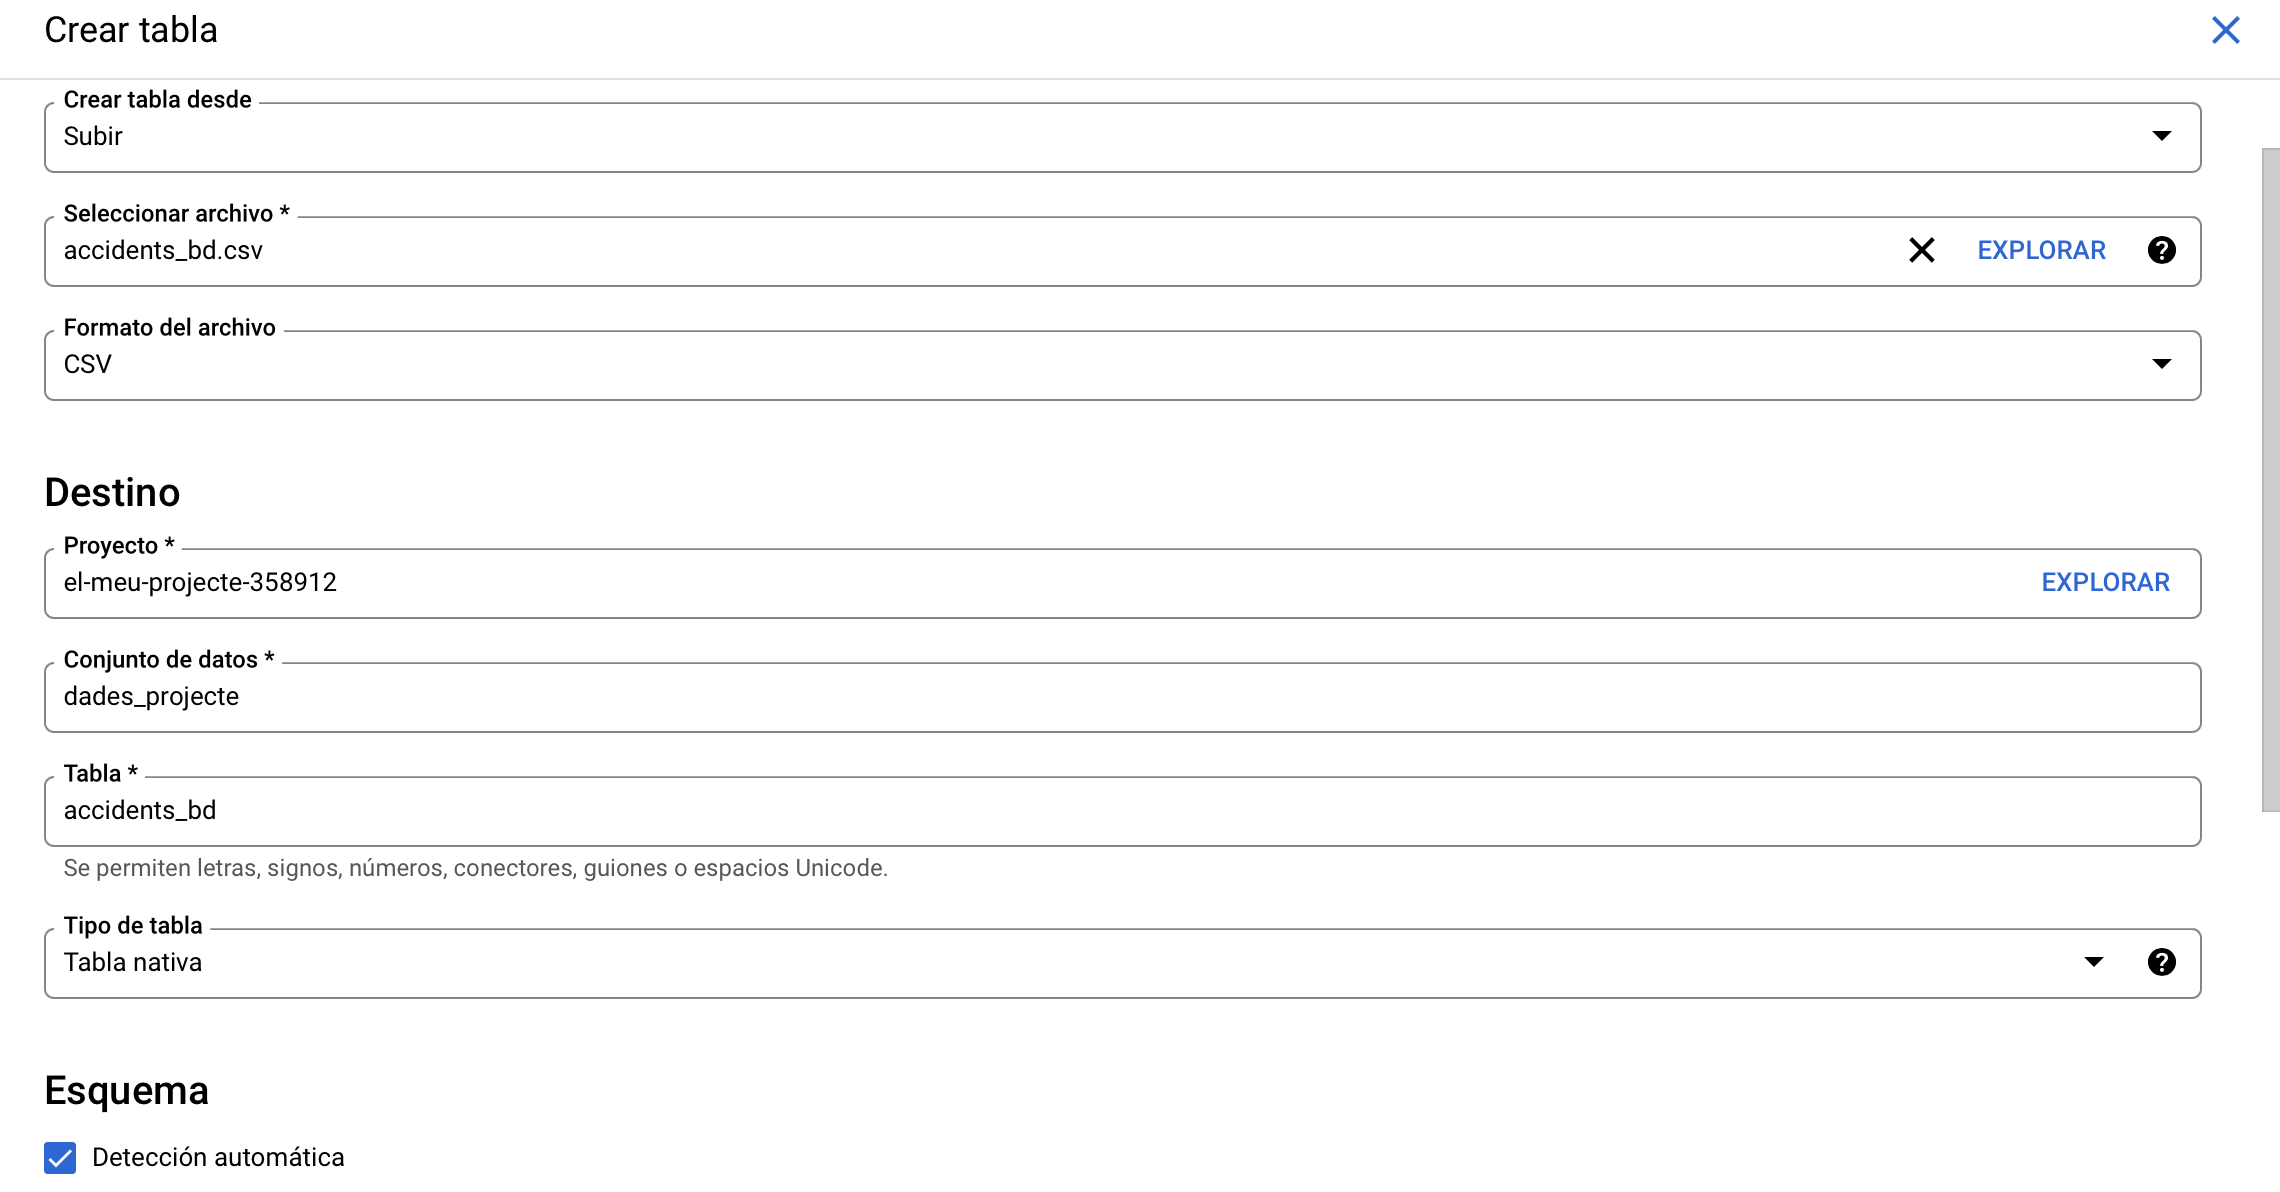
\includegraphics[width=7.25cm]{bq12}}%
\hfill
\raisebox{-.5\height}{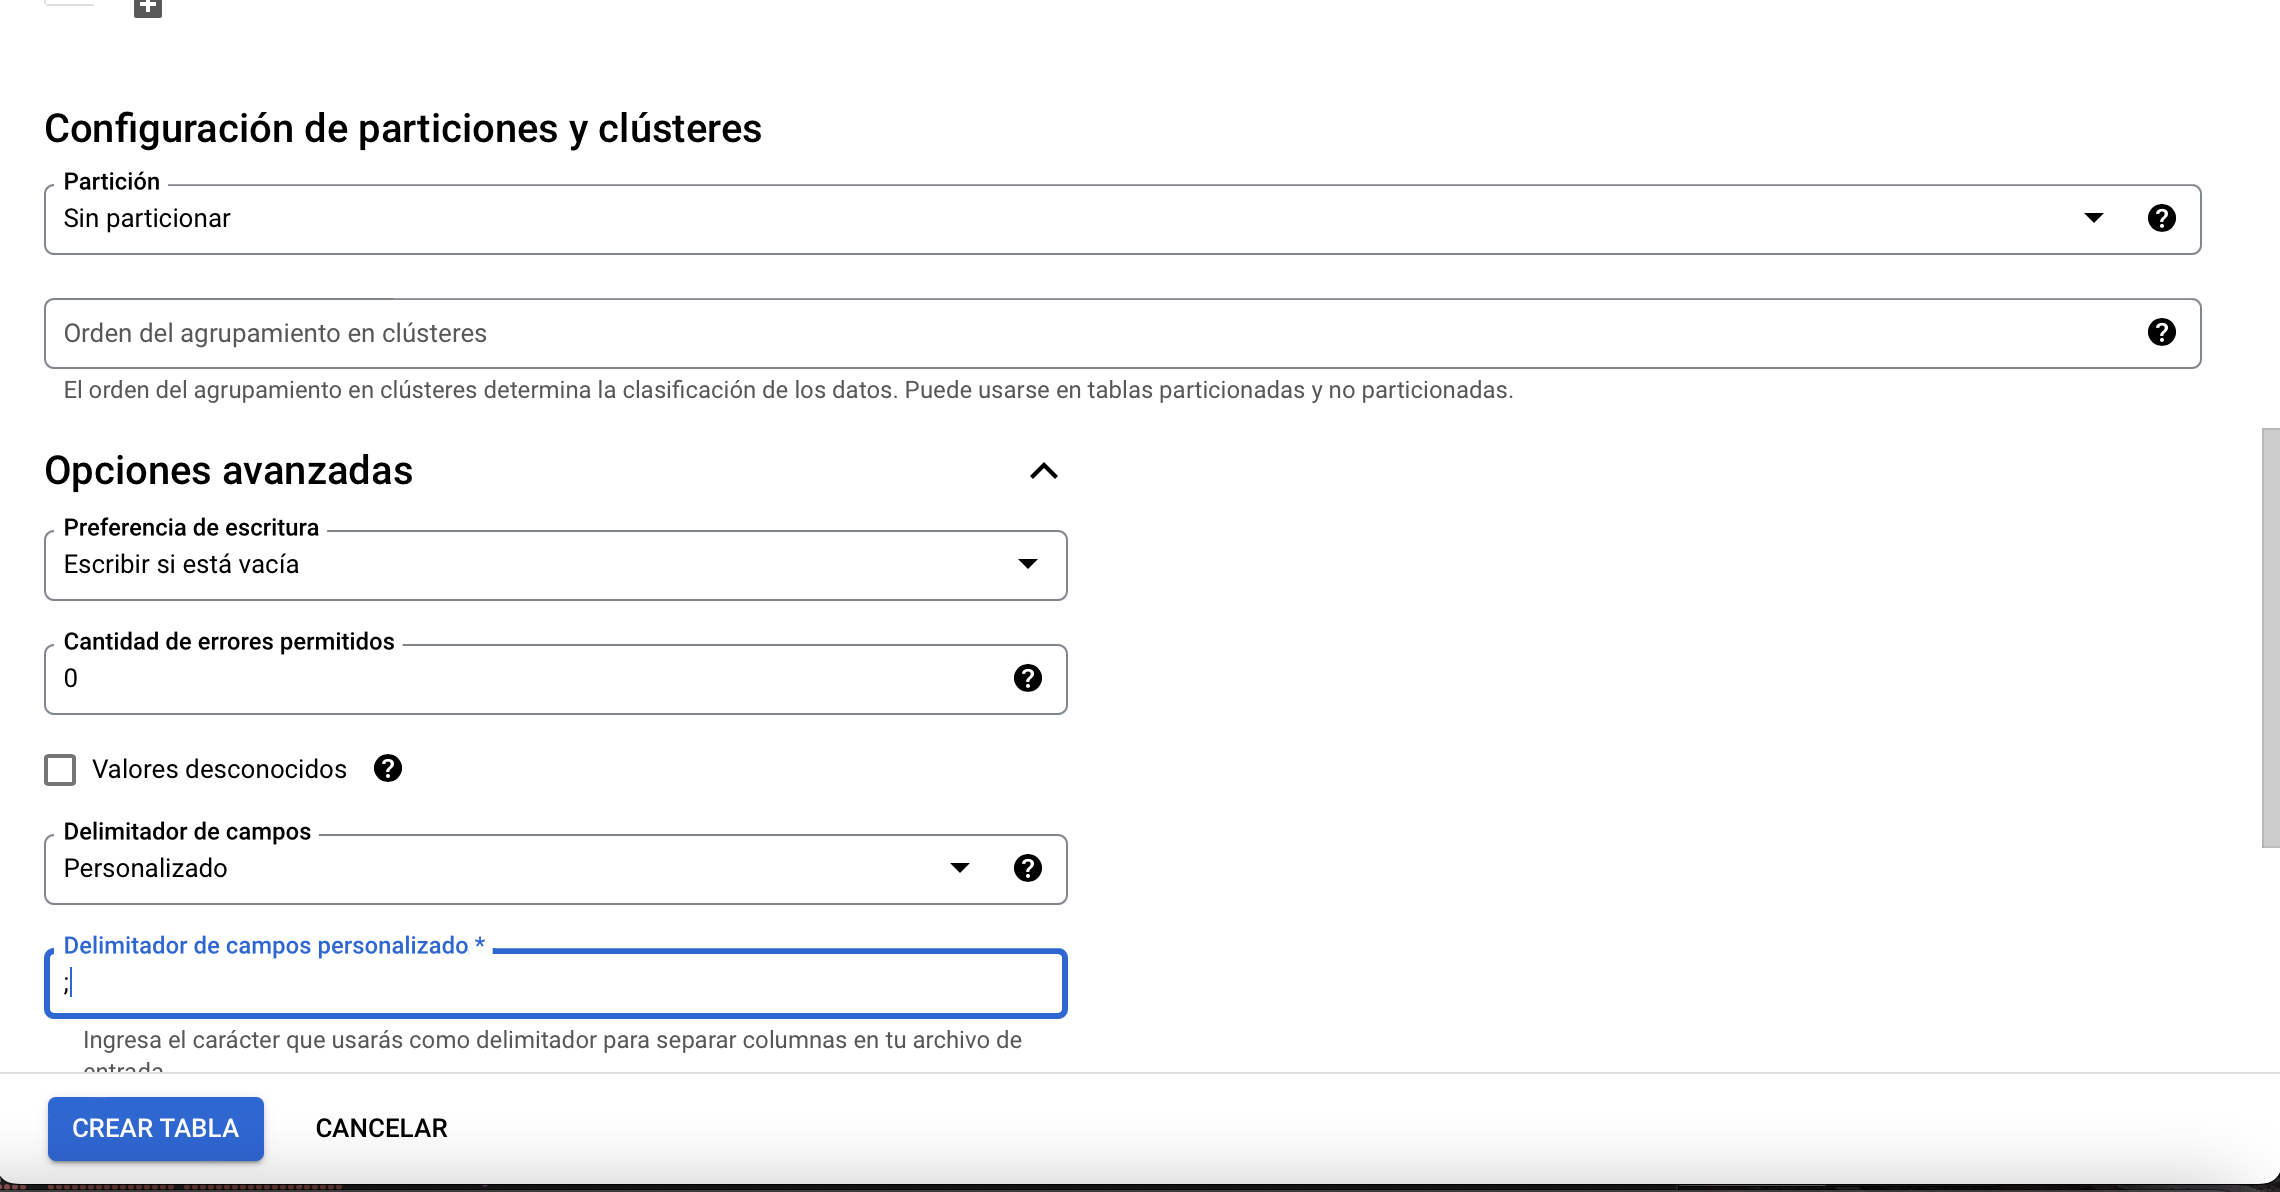
\includegraphics[width=7.25cm]{bq13}}%
\par

\caption{Lectura d'un arxiu extern}
\label{fig:bq12}
\end{figure}
\vspace{2mm}

Quant al projecte i al conjunt de dades, els deixarem com estan. I després, el nom de la taula, \verb|accidents_bd|, farà saber que inclou informació sobre diversos accidents de trànsit. A continuació, tenim l'opció de definir explícitament l'esquema. No obstant això, atès que es tracta d'un arxiu CSV amb múltiples columnes, podem triar l'opció de detectar automàticament. D'aquesta manera, BigQuery donarà un cop d'ull al contingut de cada columna i determinarà quin ha de ser l'esquema. Més enllà d'això, al final de la finestra de creació de la taula ens apareixeran unes Opcions avançades. Aquestes opcions permeten la lectura de diferents tipus de CSV, entre d’altres coses. Sabem que el delimitador de camps d’un CSV pot ser una tabulació o una coma entre d’altres possibilitats. En el nostre cas, cal especificar que el nostre tabulador és el punt i coma “;”. Si hem establert totes aquestes especificacions, ja podrem començar amb l’anàlisi.

\vspace{2mm}

Ara es pot comprobar que \verb|accidents_bd| apareix sota el conjunt de dades \verb|dades_projecte|. A continuació, podem accedir a la informació de la taula i al seu contingut desplegant el menú i triant Obrir. En l'esquema de la taula, sabrà que s'ha detectat automàticament el tipus dels diferents camps. Donem un cop d'ull als detalls de la taula. Aquí notaràs que la grandària total és de poc més de 280 KB. El nombre de files és d'unes 2.780. I després, quan ens dirigim a la Vista Prèvia, obtenim un cop d'ull als continguts. 

\subsection{Consulta de dades i visualització d'estadístiques de consultes}

Ara, per a executar consultes en aquesta taula, ens dirigim al botó de consulta. Això ens permetrà obrir una nova pestanya de consulta. Aquesta pot ser una pestanya completament nova que ocultarà aquesta vista de detalls, mentre que una pestanya dividida ens permetrà fer referència a aquesta vista de detalls per a la taula mentre construïm una consulta. Observarà que ha aparegut una nova pestanya cap a la dreta, i que la consulta per defecte que apareix aquí inclou una clàusula SELECT però no hi ha camps després de SELECT. Precisament per això hi ha un error de sintaxi. Ara, per a completar la clàusula SELECT, podríem escriure els noms dels camps, o bé BigQuery inclou aquesta funció en la qual podem seleccionar els camps des de la vista de l'esquema. Per exemple, podem fer la consulta més bàsica a la base de dades, que ens retornarà la taula sencera:

\begin{verbatim}
SELECT *
FROM `[nom_projecte].[nom_base_de_dades].[nom_taula]`
LIMIT 1000
\end{verbatim}

\vspace{2mm}

Executarem aquesta consulta prement Executar. Els resultats han aparegut, i aquesta consulta s'ha executat en uns 0,3 segons per a mi. Per descomptat, podem desplaçar-nos i donar un cop d'ull a tots els resultats. No obstant això, el que és més interessant si ets nou en BigQuery són els detalls addicionals en el panell inferior. En concret, si ens dirigim a la secció d'Historial Personal, podem donar un cop d'ull als diferents treballs que s'han creat per a cada operació que hem realitzat. Per exemple, cada treball es classifica com QUERY si es realitza un SELECT o fins i tot un INSERT. Després es pot registrar una operació LLOEU per a quan carreguem les dades de l'arxiu CSV. Aquesta interfície sí que ens permet accedir a informació addicional per a cadascun dels treballs. Per exemple, si es mostren els detalls de l'últim treball creat, podem veure el que BigQuery ha fet per nosaltres per a assegurar-se que aquesta consulta s'executi i retorni els resultats. Aquí podem veure l'usuari que va iniciar aquest treball, quan es va crear exactament el treball, quan va començar i va acabar, i el més important, el nombre de bytes processats i el nombre de bytes facturats. Aquí podràs observar que el nombre de bytes facturats és de 10 megaoctets, que és de fet la quantitat mínima facturada per a cada consulta per Google Cloud Platform amb la finalitat de tenir en compte les despeses generals. Per a consultes més realistes que impliquin diversos megaoctets, o fins i tot gigaoctets, els bytes processats i els bytes facturats seran bastant similars. Sortint d'aquesta vista, passem a l'Historial del Projecte, que ens donarà els detalls dels treballs de tot el projecte i no sols del nostre propi usuari. I després està la secció de Consultes Guardades. Aquí és on es pot accedir a les consultes que hàgim guardat, encara que aquestes apareixeran en el menú de l'Explorador al costat dels nostres projectes i conjunts de dades.

\vspace{2mm}


Si escrivim a l’editor la nostra consulta, apareixerà un validador d’aquesta a la part superior dreta de la finestra. Aquest validador pot agafar dues formes:
- Si la consulta és vàlida, apareixerà un icona de verificación verd.
- Si la consulta no és vàlida, aparaixerà un icona d’exclamació Vermell
A més, el validador també mostra la quantitat de dades que la consulta processarà quan s’executi. Per exemple, si demanem en una consulta que ens retorni una columna selncera, el validador de la dreta ens marca que es processaran una quantitat de gairebé 22KB, tal i com es pot veure a la figura ~\ref{fig_bq16}.

\vspace{2mm}
\begin{figure}[h!]
\begin{center}
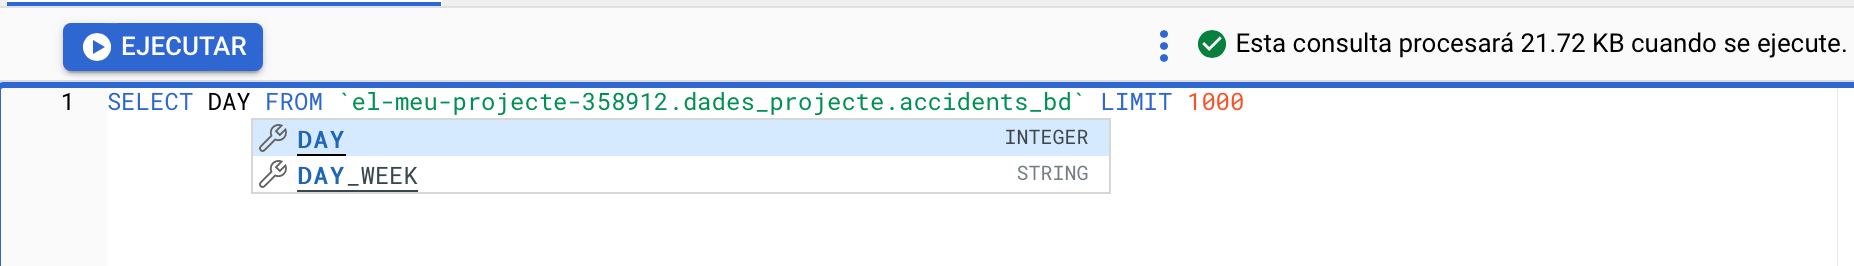
\includegraphics[width=10cm]{bq16}
\end{center}
\caption{Exemple del funcionament del validador de consultes}
\label{fig:bq16}
\end{figure}
\vspace{2mm}

\subsection{Creació d'una taula a partir d'un resultat de consulta}

Després d'haver introduït dades de fonts externes en BigQuery. Ara veurem com podem crear noves taules a partir de les existents. En concret, la taula en l'Editor de Consultes. Ara he inserit una consulta que selecciona una sèrie de camps diferents, incloent-hi el nom, la companyia, el gènere i el director de la taula en el conjunt de dades. Es tracta de pel·lícules el pressupost de les quals és superior a 100 milions de dòlars. L'objectiu és crear una nova taula a partir dels resultats d'aquesta consulta concreta. Aquí apliquem un filtre, no sols eliminant els rols a causa de la clàusula where i seleccionant només camps específics. Però vostè notarà en línia número dos que també creguem una nova columna anomenada benefici, que es computa mitjançant el càlcul de la diferència entre el creixement de les pel·lícules. És a dir, la quantitat de diners que va ingressar i després restant el pressupost d'aquesta. Per descomptat, per a veure el cost associat a aquesta consulta. Podem minimitzar l'Explorador. I ara sabem que encara que el cost calculat apareix com 492 kilobytes en aquest cas. El cost real serà de 10 megaoctets que és el mínim per a BigQuery. Quan executem això, els resultats apareixen i hi ha un total de 315 files de dades. Ara hem d'exportar totes aquestes dades a una nova taula. Revisa algunes de les opcions d'exportació. Podem donar un cop d'ull al menú Guardar resultats. Vostè observarà que hi ha un nombre de diferents opcions aquí per a la manera de guardar els resultats. Podem guardar-los com un arxiu CSV en Google Drive o en un arxiu local. El format JSON també està disponible com una opció d'exportació. No obstant això, el que oferirem aquí és exportar el contingut a una nova taula de BigQuery. Una vegada feta aquesta selecció, podem decidir el nom del projecte i el conjunt de dades on s'aprovisionarà la taula i després establir un nom de taula. La cridaré simplement. Llavors, quan guardem les coses, això haurà iniciat un nou treball per a aprovisionar la nova taula i carregar-la amb dades. Una vegada que tanquem aquesta notificació, podem treure el pin de l'Explorador i baix, apareix com una taula. En obrir-la confirmem que l'esquema apunta a les mateixes columnes que havíem referenciat en la clàusula select de la consulta que va crear aquesta taula, encara que hi ha una columna anomenada profit el tipus de la qual s'ha establert com un enter. Des dels detalls podem confirmar que el nombre de files coincideix amb el dels resultats de la consulta, concretament 315. I després la vista prèvia ens mostrarà quins són exactament les dades. Desplacem-nos i confirmem que la columna de beneficis es deriva, efectivament, del creixement i del pressupost. Quin és llavors la finalitat d'aquesta taula? Bé, atès que només conté un subconjunt de la taula original. Significa que les consultes contra això tindran potencialment menys dades per a processar que les consultes que s'executen directament contra. Si només volem analitzar les pel·lícules de gran pressupost amb un pressupost de més de 100 milions, és millor executar les nostres consultes en aquesta taula més petita, que inclou tota la informació que necessitem i probablement tindrà un cost de consulta menor. Per a executar una consulta d'aquest tipus, obrirem l'Editor de Consultes i a substituir aquesta consulta directament contra per aquesta altra que es dirigeix a la taula recentment creada. Observarà que els camps de la clàusula select són idèntics als quals teníem anteriorment, però la clàusula where és una mica diferent. I mentre que la consulta anterior va processar 492 kilobytes, aquesta només funcionarà amb 34,7. Seguim endavant i executem aquesta consulta. I els resultats confirmen que les consultes contra aquesta taula funcionen com s'espera que ho facin.

sèrie temporal de 31 observacions, on per cada dia digui el nombre d’accidents ocorreguts amb víctimes.

\begin{verbatim}
SELECT DAY, COUNT(*) AS FREQ
FROM `level-oxygen-353005.examen_final.accident`
GROUP BY DAY
\end{verbatim}

\vspace{2mm}
\begin{figure}[h!]
\par
\raisebox{-.5\height}{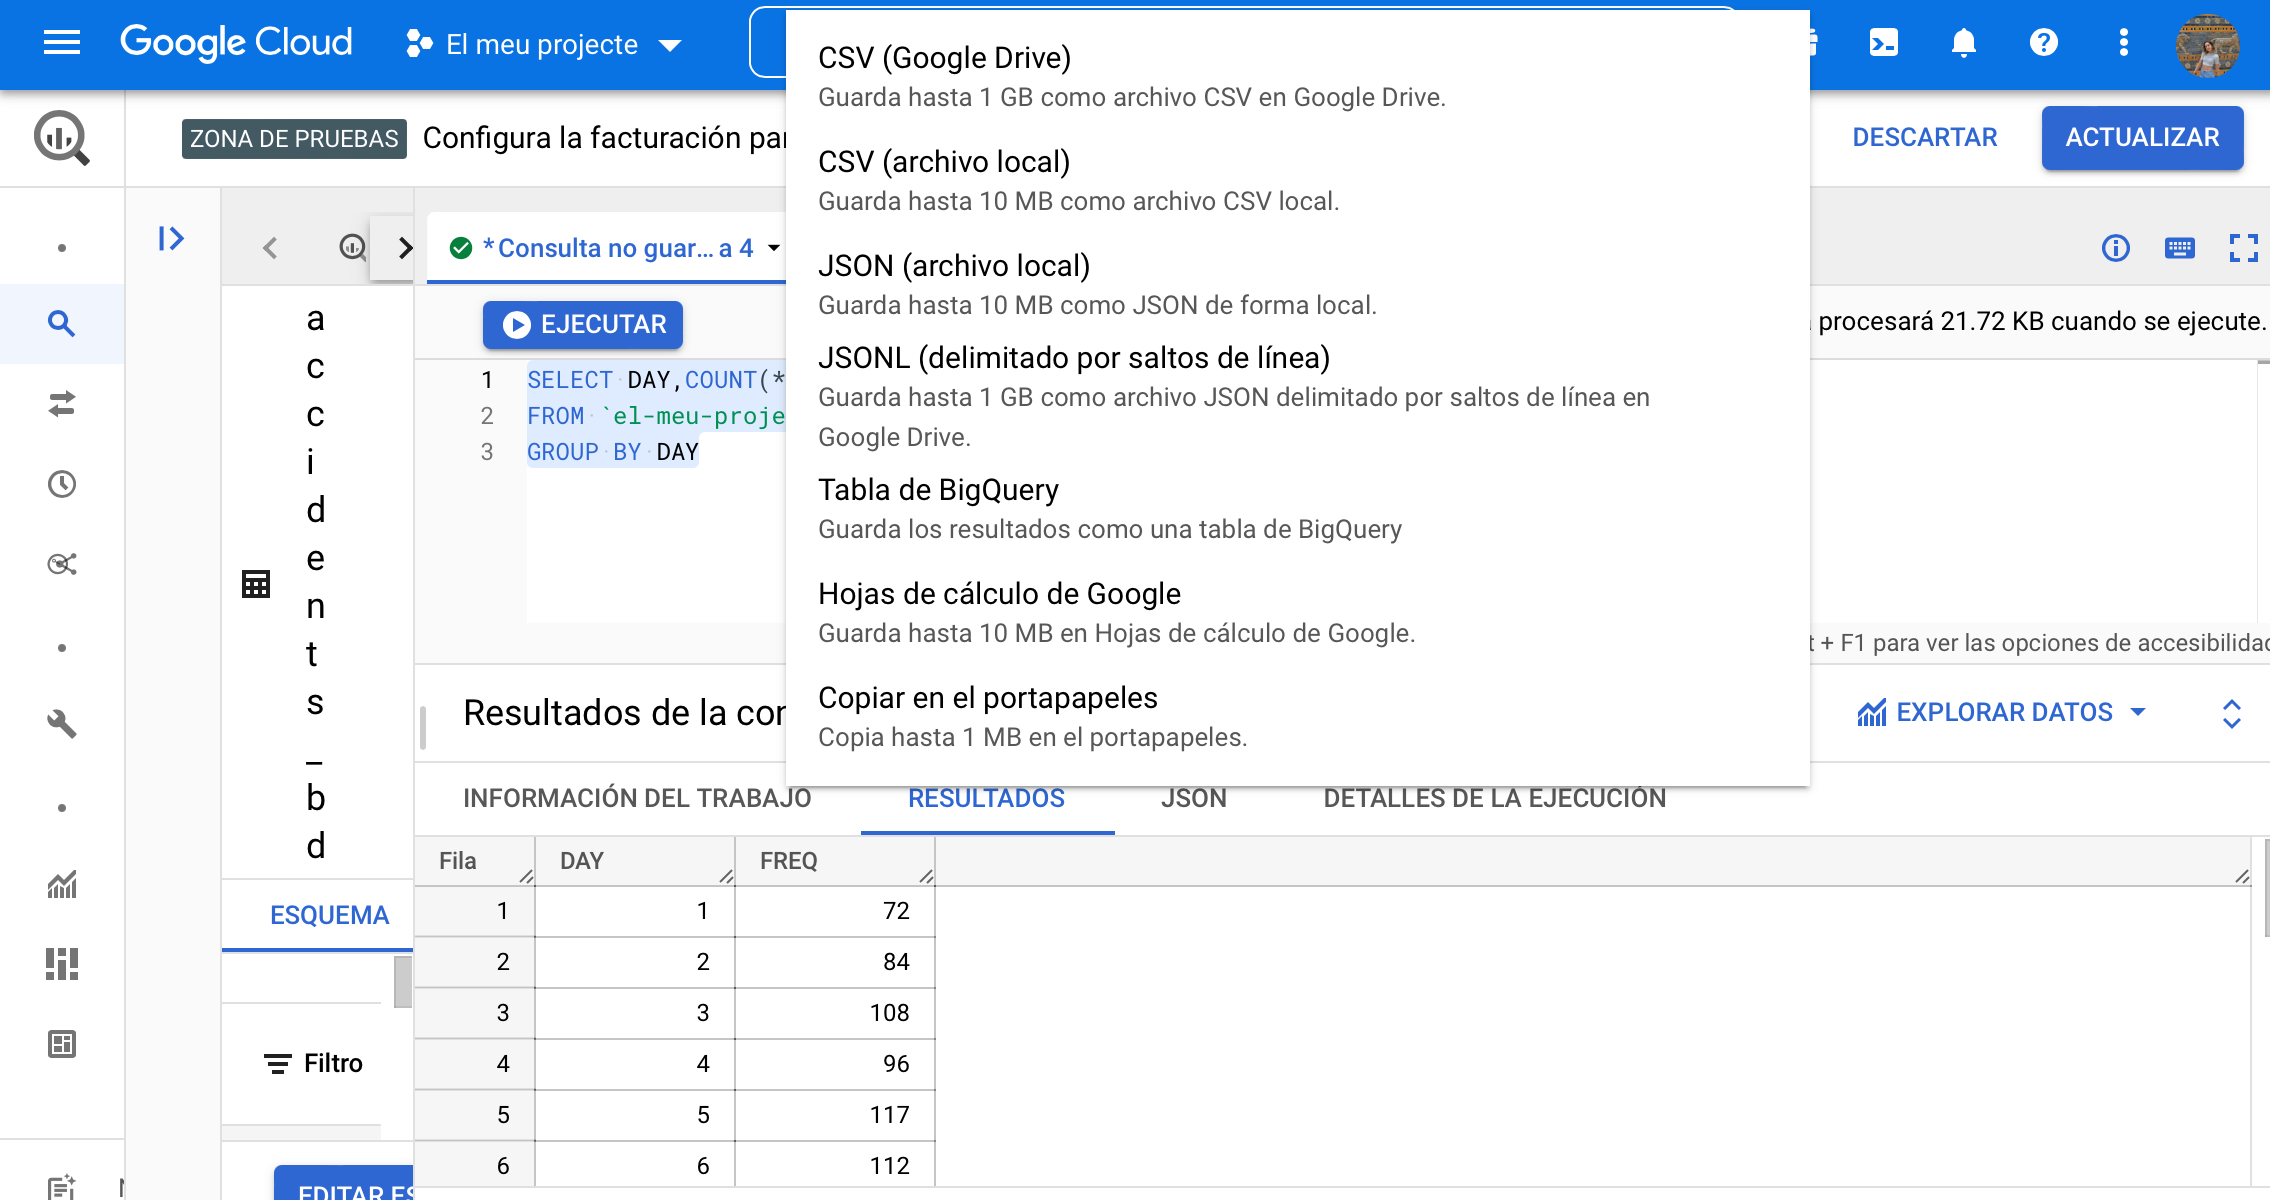
\includegraphics[width=7.25cm]{bq17}}%
\hfill
\raisebox{-.5\height}{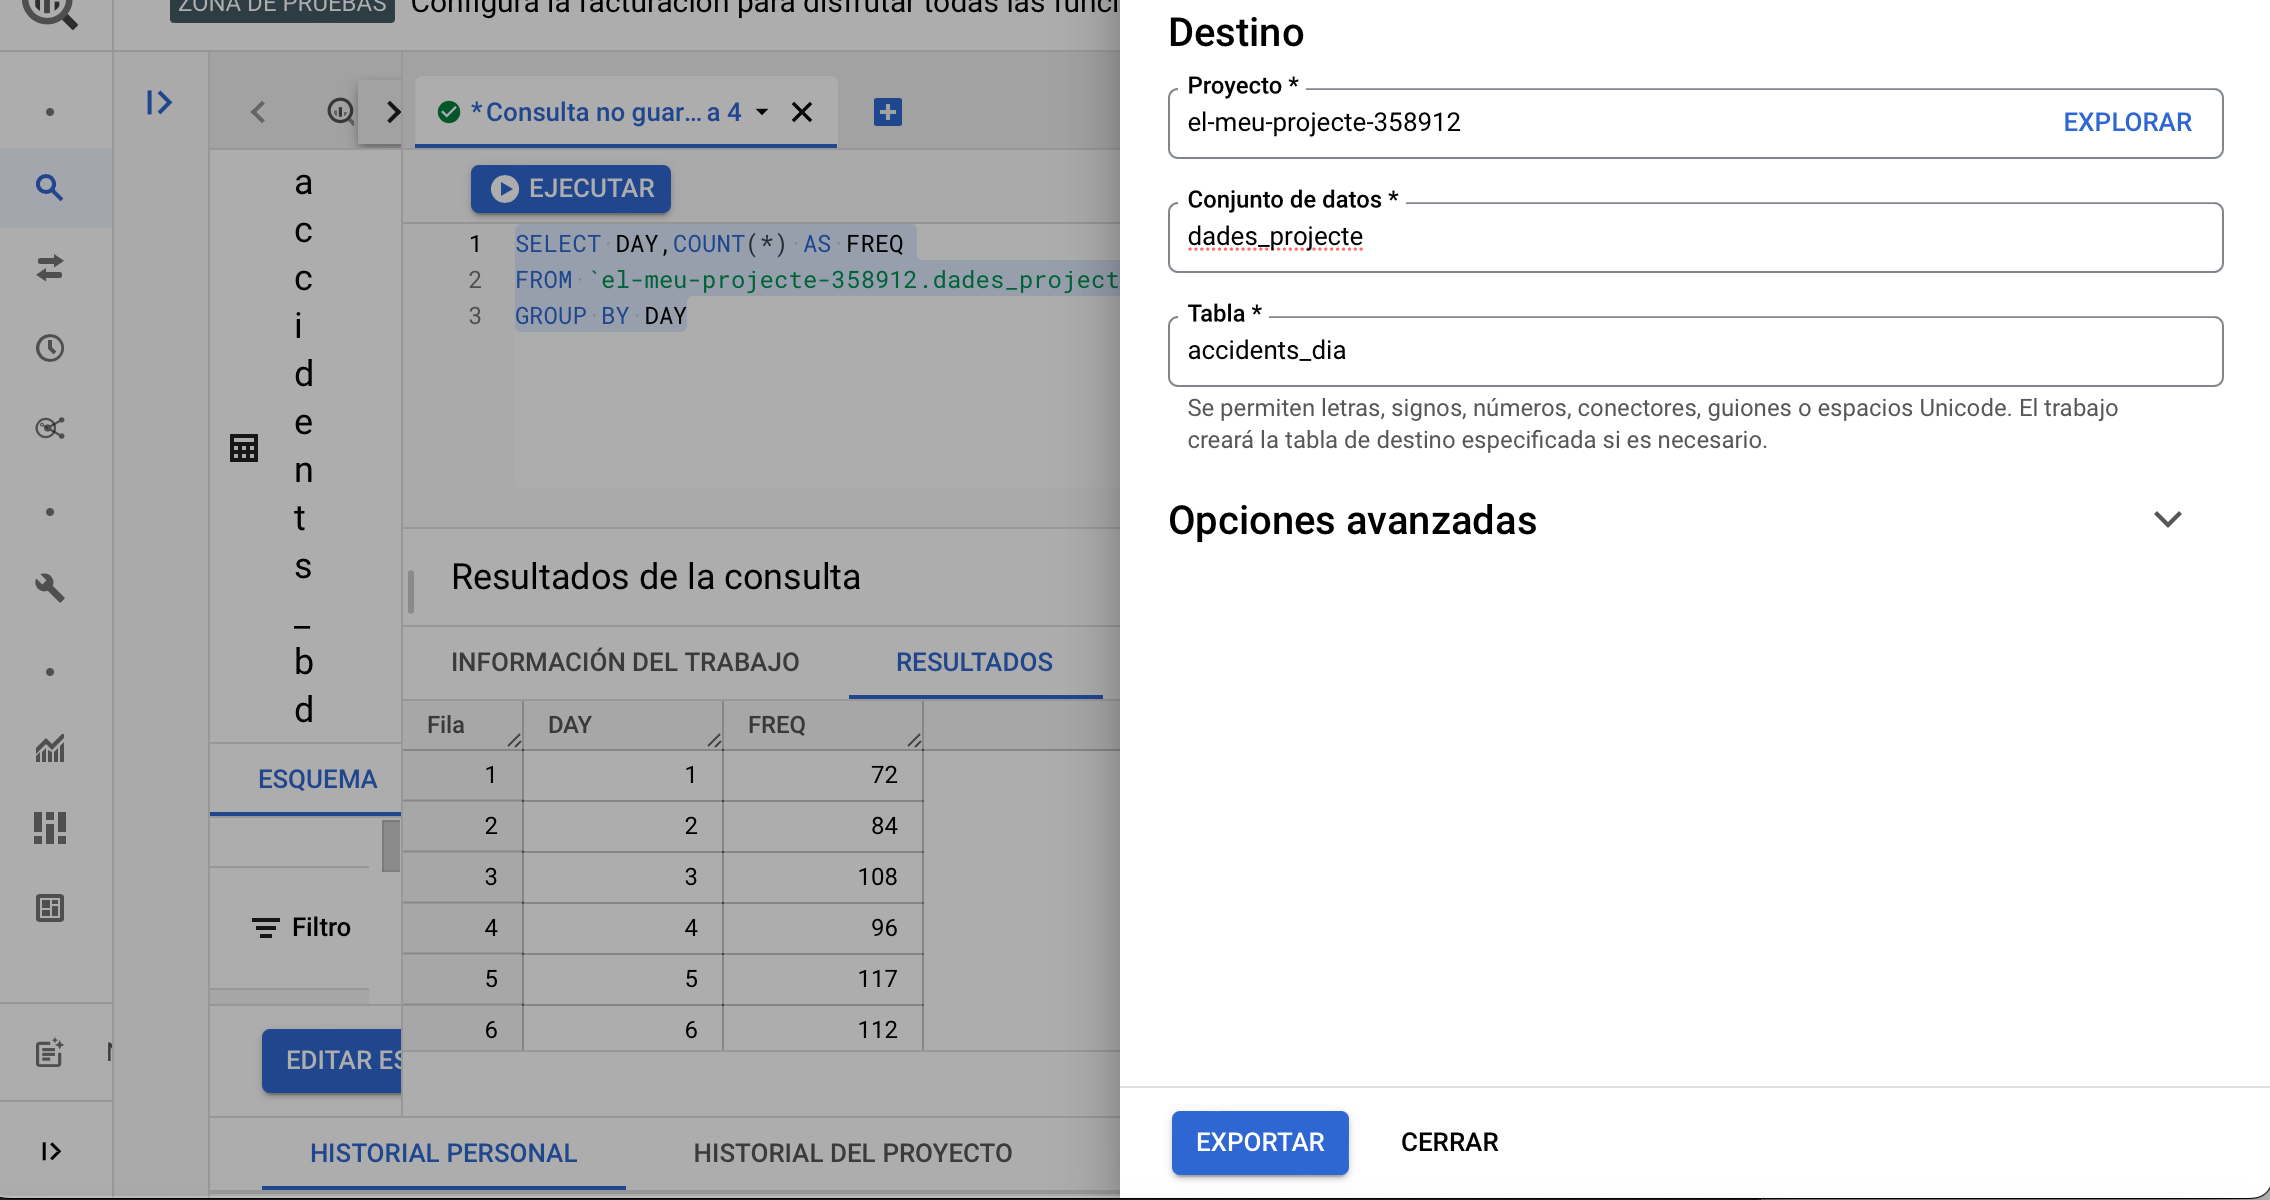
\includegraphics[width=7.25cm]{bq18}}%
\par

\caption{Creació d'una taula a partir d'una consulta}
\label{fig:bq17}
\end{figure}
\vspace{2mm}


\newpage

\section{Execució de consultes i visualització de resultats}

\subsection{Conjunts de dades públics a BigQuery}

\subsection{Configuració i ús de memòria cau de BigQuery}

\subsection{Taules externes de BigQuery}

\subsection{Integració de BigQuery amb Data Studio}

\newpage

\listoffigures


\end{document}
